\documentclass[supercite]{HustGraduPaper}
%进行个人信息设置
\title{RIS辅助的无线通信系统的原型验证} %论文题目
\author{裴熙隆} %作者姓名
\date{\today} %日期,默认当日
\school{人工智能与自动化学院} %院系名称
\classnum{自动化1705班} %专业班级
\stunum {U201714286} %学号
\instructor{陈忠、尹海帆} %指导教师姓名

%添加自己要用的其他宏包
\usepackage{xltxtra}
\usepackage{bm}
\usepackage{array}
\usepackage{multirow}
\usepackage[caption=false,font=footnotesize]{subfig}
\usepackage{algorithm}
\usepackage{algorithmic}
\usepackage{amsthm}
\usepackage{color}
\usepackage{listings}
\usepackage{xcolor}

\newtheorem{theorem}{\indent 定理}[section]
\newtheorem{lemma}{\indent 引理}[section]
\newtheorem{proposition}{\indent 命题}[section]
\newtheorem{corollary}{\indent 推论}[section]
\newtheorem{definition}{\indent 定义}[section]
\newtheorem{example}{\indent 例}[section]
\newtheorem{remark}{\indent 注}[section]
\renewcommand{\proofname}{\indent\bf 证明}

\begin{document}
%生成标题页 \maketitle[可选参数]\end{document}\end{document}
%可选参数:
%logo color=green/black 华中科技大学字样的颜色,绿色或者黑色,默认绿色
%line length=12em 填写信息处横线的长度,默认12em
%line font=huawenzhongsong 填写信息的字体,默认huawenzhongsong
\maketitle

%生成声明与授权书页 \statement[可选参数]
%可选参数:
%confidentiality=yes/no/true/false/empty
%是否保密,yes/true为保密;no/false为不保密,empty为不填,默认为empty
%year=5 保密年数,默认为空
\statement[confidentiality = false]

\clearpage %结束上一页
\pagenumbering{Roman} %摘要页码为大写罗马数字

%填写中文摘要内容和关键字
\begin{cnabstract}{可重构智能表面;智能反射面;无线中继;大规模多进多出系统;原型系统;现场可编程逻辑门阵列}
	%请注意使用中文分号“;”分割关键词!

	作为最新一代蜂窝移动通信技术,第五代移动通信技术(5G)以其大带宽、低时延、大连接等特性,将为物联网、社交娱乐、智慧交通、工业互联网等技术发展注入新的活力,助力我国数字经济发展。
	但现阶段 5G 以及毫米波的应用还存在覆盖差、成本高、能耗高等痛点问题。
	近年来,人们研制出了能够对撞击的无线电波进行特定变换的基于电磁的可重构结构,它们的工作频段非常广阔,可以覆盖 Sub-­6 GHz、毫米波甚至太赫兹。
	可重构智能表面(也被称为智能超表面)是一种具有大量无源元件的二维结构,近年来被认为是实现节能智能无线通信的革命性技术之一。

	本文中,首先用少量篇幅介绍了电磁超表面的相关基础理论,包括广义反射定律和折射定律以及智能超表面对电磁波的调控机理的理论。
	并对设计的RIS通信系统建模分析,解释了无源金属表面如何散射入射波,然后推导出智能超表面必须如何设计来模拟这种表面,同时控制散射波的方向性,总结了一个严格的路径损耗模型。
	之后建立智能超表面系统的传输模型,解释了在何种条件下,系统达到最大传输速率。
	
	本设计中,我们开发了一种新型的高增益低成本智能超表面通信系统,其核心部件RIS具有256个元件。
	该原型由模块化硬件和灵活的软件组成,包括以下内容:
	数据交换主机、用于基带和射频信号处理的通用软件无线电外设,以及用于信号传输和反射的RIS,
	系统还包括一些附加组件如喇叭天线,变频器,相控阵天线。
	文章着重介绍了控制电路的设计和驱动、固件的设计。
	最后的测试结果表明系统能实现波束调控,达到了设计目的。

\end{cnabstract}
%填写英文摘要内容和关键字
\begin{enabstract}{Reconfigurable intelligent surface; intelligent reflecting surface; wireless repeating; massive multiple-input multiple-output; prototype; field programmable gate array}
	%Please Use English Semicolon and a Space "; " to Separate Keys! 

	As the latest generation of mobile communication technology, the fifth-generation mobile communication technology (5G) will be injected into the Internet of Things, Social Entertainment, Smart Transportation, Industrial Internet, and other technologies in its large bandwidth, low delay, and large connectivity.
	This technology will help China's digital economic development.
	However, the application of 5G and millimeter-wave at this stage also has some painful problems with high cost, high energy consumption, and poor coverage.
	In recent years, people have developed electromagnetic-based reconfigurable structures that can be used for a radio wave impacted, and their operating frequency bands are very broad, including Sub-6 GHz, millimeters, or even terahertz.
	Reconfigurable intelligent surfaces (RISs) are two-dimensional structures having a large number of passive components, which is considered to be one of the revolutionary techniques to achieve energy-saving intelligent wireless communication.
	
	In this article, the basic theory of the intelligent reflecting surface is first introduced.
	Then, we analyze the model of the RIS communication system, explained how to scatter incident waves on the passive metal surface.
	Furthermore, we summarize a strict path loss model.
	We build the transmission model of the RIS system, explain the system reaches the maximum transmission rate in what condition.

	In this design, we have developed a new type of high gain low-cost RIS communication system with 256 components. This prototype consists of modular hardware and flexible software, including the following: data exchange hosts, universal software radio peripherals for baseband and RF signal processing, and the RIS for signal transmission and reflection, the system also includes some additional components such as a horn antenna, a frequency converter, an active array antenna. The article focuses on the design of the control circuit and the firmware. The final test results indicate that the system can achieve beam regulation and achieve design purposes.

\end{enabstract}

%生成目录 \tableofcontents[可选参数]
%可选参数:
%pagenum=yes/no/true/false 目录是否显示页码,默认为false
%toc in toc=yes/no/true/false 目录中是否有目录及其页码,默认为false
%level=4 目录级数,默认是4,即显示到subsubsubsection
%section indent=0em 目录第一级的缩进,默认是0em
%subsection indent=1.5em 目录第二级的缩进,默认是1.5em
%subsubsection indent=3.8em 目录第三级的缩进,默认是3.8em
%subsubsubsection indent=7em 目录第四级的缩进,默认是7em
%paragraph indent=11em 目录第五级的缩进,默认是11em
%subparagraph indent=13em 目录第六级的缩进,默认13em
%indent=normal/noindent/hustnoindent/sameforsubandsubsub 快速缩进设置,具体见文档
%dot sep=4.5 目录点间距,默认4.5
%section dot sep=4.5 目录第一级的点间距,默认是4.5
%subsection dot sep=4.5 目录第二级的点间距,默认是4.5
%subsubsection dot sep=4.5 目录第三级的点间距,默认是4.5
%subsubsubsection dot sep=4.5 目录第四级的点间距,默认是4.5
%paragraph dot sep=4.5 目录第五级的点间距,默认是4.5
%subparagraph dot sep=4.6 目录第六级的点间距,默认是4.5
%请注意在合适的位置放置\pagenumbering{numstyle}使用新的页码
\tableofcontents

\clearpage%结束上一页
\pagenumbering{arabic} %正文页码为阿拉伯数字

%正文内容从这里开始
\section{绪论}
%这是小四号的正文字体,段间距1.5倍
%通过空一行实现段落换行,仅仅是回车并不会产生新的段落
%\par 也可以通过\verb|\par|命令来新起一段

\subsection{引言}

作为最新一代蜂窝移动通信技术,第五代移动通信技术(5G)以其大带宽、低时延、大连接等特性,将为物联网、社交娱乐、智慧交通、工业互联网等技术发展注入新的活力,助力我国数字经济发展。
目前,增强移动宽带(eMBB)、高可靠低时延(uRLLC)和海量机器类通信(mMTC)成为5G的三大应用场景。进一步细分,在3D超高清视频、云工作/娱乐、AR/VR、工业自动化、关键任务应用、自动驾驶、ITU-R WP5D、智慧城市和智能家居/建筑等方方面面都有长足的应用。
这是因为5G有着多项关键技术,其中举足轻重的就是毫米波(Millimeter Wave)技术和大规模多入多出(Massive MIMO)技术;前者可以增加带宽资源,提供更低的时延,并且天线尺寸更小,可以使设备轻量化,从而部署更为便捷,后者可以提高频谱效率。
5G毫米波技术频率资源丰富、带宽大、峰值速率极高,有时延低和容量大的优点,这是5G毫米波系统的最大优势之一,适用于大量4k/8k视频业务的场景\cite{8732419}。

具体来说,毫米波或极高频(Extremely high frequency, EHF)是指波长短于超高频(SHF)的电磁波,它的波长由1 mm到10 mm,所对应的频率范围是30~300 GHz\cite{enwiki:1021979549}。
现阶段主要毫米波应用于气象雷达、空间通信、射电天文等方面。
在5G通信中,美国已率先启用毫米波频段,其毫米波部署最为广泛,AT\&T、Verizon和T-Mobile从2018年起陆续在美国国内的城市开通利用毫米波频谱的5G商用网络,而中国现在部署的主要是Sub-6 GHz频段\cite{ZTE2020}。
中国的三大运营商从2017年开始就不断联合各厂家进行了5G毫米波的关键技术测试和验证,随着2020年3月工信部推动5G加快发展的通知以及2022年冬奥会毫米波应用场景的预期,毫米波大规模商用的脚步越来越近\cite{ZTE2020}。
最近中新社报道称,5G毫米波将赋能北京2022年冬奥会。可以想象,有了毫米波技术的加持,这一届冬奥会会给我们带来不一样的精彩。

但现阶段5G以及毫米波的应用还存在覆盖差、成本高、能耗高等痛点问题。由于频点较高,毫米波呈现准光学传播特性,穿透能力很弱,绕射、散射很不明显。
如\autoref{tab:Loss-contrast}所示,毫米波容易收到大尺寸结构的阻挡,生活中高楼、墙面、混凝土、钢筋、玻璃、人体等物体的阻挡会造成信号衰减严重,在极端情况下,26 GHz毫米波于3.5 GHz的穿透损耗高90 dB,大雨等恶劣天气也会对毫米波的覆盖产生较大的影响\cite{8732419}。
另外,人体的遮挡在极高频时也会有不可忽视的影响。
从上述的毫米波的传播特性来看,它适用于室内室外的视距(Line-of-sight, LoS)通信,而不适用于室内外有较高的穿透损耗的场景。
如\autoref{fig:Overlay-comparison}为在城市中模拟的3.5 GHz和26 GHz两种频段的覆盖范围对比。
从右图可以看到,对于视距场景,毫米波覆盖尚可;而被遮挡的区域就差强人意了。
我们以参考信号接收功率(Reference Signal Receiving Power, RSRP)不低于-110 dBm为基准,26 GHz的总体覆盖(按面积计算)只能达到 3.5 GHz 的62\%\cite{ZTE2020}。

\begin{generaltab}{3.5 GHz和26 GHz下不同材料的穿透损耗(dB)对比\cite{ZTE2020}}{tab:Loss-contrast}
	\begin{tabular}{ccccccc}
		\toprule
		        & 混凝土 &  木头  & 雨衰(10 mm/hr) & 人体损耗 & 普通多层玻璃 & IRR玻璃 \\ \midrule
		3.5 GHz & 19  & 5.27 &      0       &  3   &  2.7   & 24.05 \\
		26 GHz  & 109 & 7.97 &     1.57     & 9-13 &  7.2   & 30.8  \\ \bottomrule
	\end{tabular}
\end{generaltab}

\begin{generalfig}[htb]{3.5 GHz和26 GHz覆盖对比\cite{ZTE2020}}{fig:Overlay-comparison}
	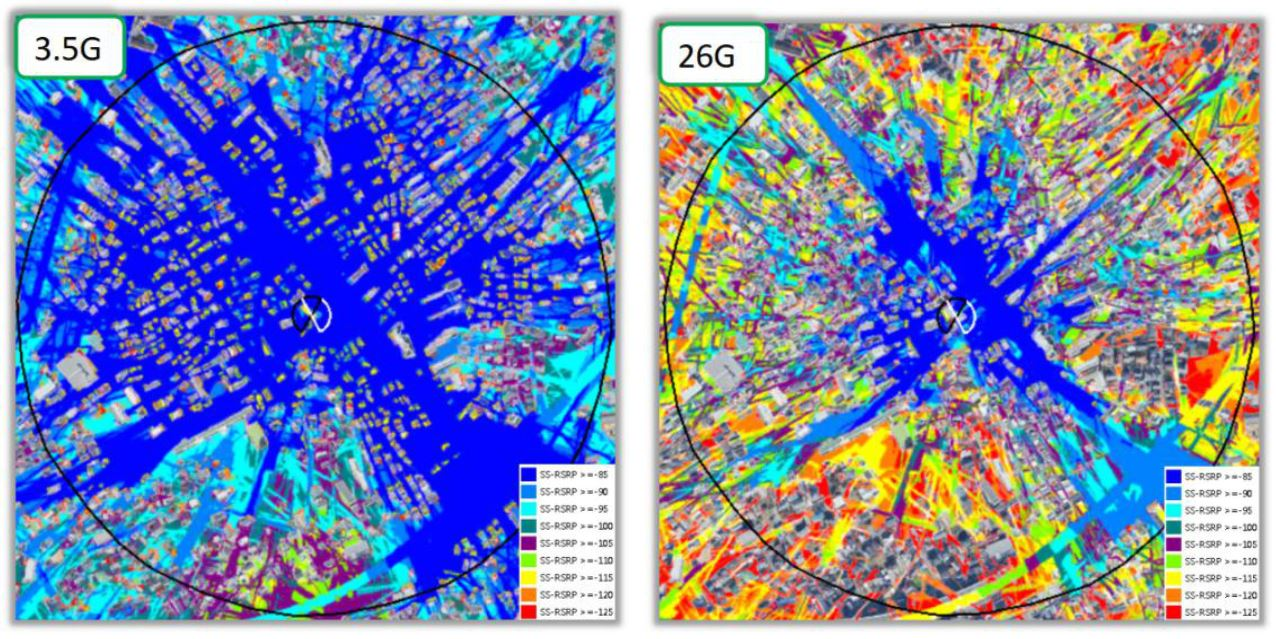
\includegraphics[width=0.8\linewidth]{Figures/Overlay-comparison.JPG}
\end{generalfig}

从毫米波设备的硬件架构来看,毫米波设备由大量的射频链路、射频开关、移相器组成用来实现模拟波束赋形。这样的收发器的组成需要所需的天线、放大器等器件相比现有通信方案增加多达数十倍,造成了成本长时间居高不下。
同时带来的也有能耗问题,复杂的射频硬件电路带来了令人难以置信的高功耗,这不是绿色通信的发展方向,也不利于实现碳中和(carbon neutrality)。

面对这些问题,急需一种能够规避高频信道不可靠性的方法,其中重要的一环便是能智能地改善当前的无线环境。
中继站是一种可以将非视距路径(Non-line-of-sight, NLoS)转化为视距路径的方法\cite{Dohler2010a}。
使用中继站传输时,需要为每个中继站配备专用的电源和射频前端,这需要很高的资本投入,而且,中继站需要先接收处理无线信号再做转发,会带来较大的时延,更为严重的是,广播出的新信号可能会干扰原信号\cite{di2020reconfigurable}。
反射阵列给出了有效的解决方案:当LoS径不能提供服务时,另一种建立替代路径的方法是通过无源非可重构镜面反射器。
反射阵列是指能够以波束的形式反射电磁波的平面\cite{huang2005reflectarray},这和曲面的反射镜不同,后者依靠物理曲率的变化决定反射波束的方向,而前者是由离散的单元组成,每个单元对应着不同的幅度和相移\cite{pozar1997design}。
无源非可重构的反射器与传统中继器相比,在成本和功耗方面有一定的优势。
但是,这种反射器的一个重大缺陷是它的反射在生产制造出来后就被固定了,在部署和使用是不可以修改的,这使得它无法适应高动态的无线信道环境。

近年来,人们研制出了能够对撞击的无线电波进行特定变换的基于电磁的可重构结构,它们的工作频段非常广阔,可以覆盖Sub-6 GHz、毫米波甚至太赫兹\cite{Wu2019}。下面将详细介绍这一新技术。

\subsection{智能超表面概述}

由于具有主动适应、改变无线通信环境的能力,可重构智能表面(RIS),也称为可重构反射阵列、可编程超表面、大型智能表面或智能反射表面,已成为无线通信研究领域的一个焦点,用于缓解在不同无线网络中遇到的各种挑战\cite{liu2020ris, huang2020holographic}。
智能超表面是由电磁材料构成的,因为它不需要改变现有的网络结构,也不需要修改现有的无线通信标准,所以特别适合“无感”地部署在建筑物外墙、公路指示牌、广告面板、车窗等平面物体上。
RIS能够通过被动反射接收信号在基站和移动用户之间形成虚拟视线链路,从而补偿长距离的功率损耗,智能地配置无线信号环境。
当基站和终端之间的直射链路被高层建筑阻断时,通过RIS的智能部署和设计,可以构建软件定义的无线环境,进而使接收信的信噪比(SINR)增强。
与传统放大转发和解码转发的中继系统相比,RIS不需要专用的大功率电源来运行,其功耗和硬件复杂度有着其他技术难以望其项背的优势\cite{di2020reconfigurable}。

2014年,中国科学院院士崔铁军教授首次提出了智能超表面并进行了实验验证,其基本结构如\autoref{fig:ris}所示\cite{cui2014coding}。
这是一种具有可编程电磁特性的二维薄层人工电磁表面结构,可以应用于从微波到可见光的各种波段中\cite{CHN_zhang2017}。
从\autoref{fig:ris}中可以看出,超表面由精心设计的电磁单元规则排列而成,这些电磁单元通常由金属铜片、电磁介质和可调元件\footnote{这里可调元件指的是变容二极管、PIN二极管、射频开关、MEMS器件等有不同状态的元件。}组成。
通过控制电磁单元中的可调元件,以可编程的方式更改反射的电磁波的电磁参数(例如幅度和相位)\cite{CHN_zhou2020}。

\begin{generalfig}[htb]{智能超表面示意图}{fig:ris}
	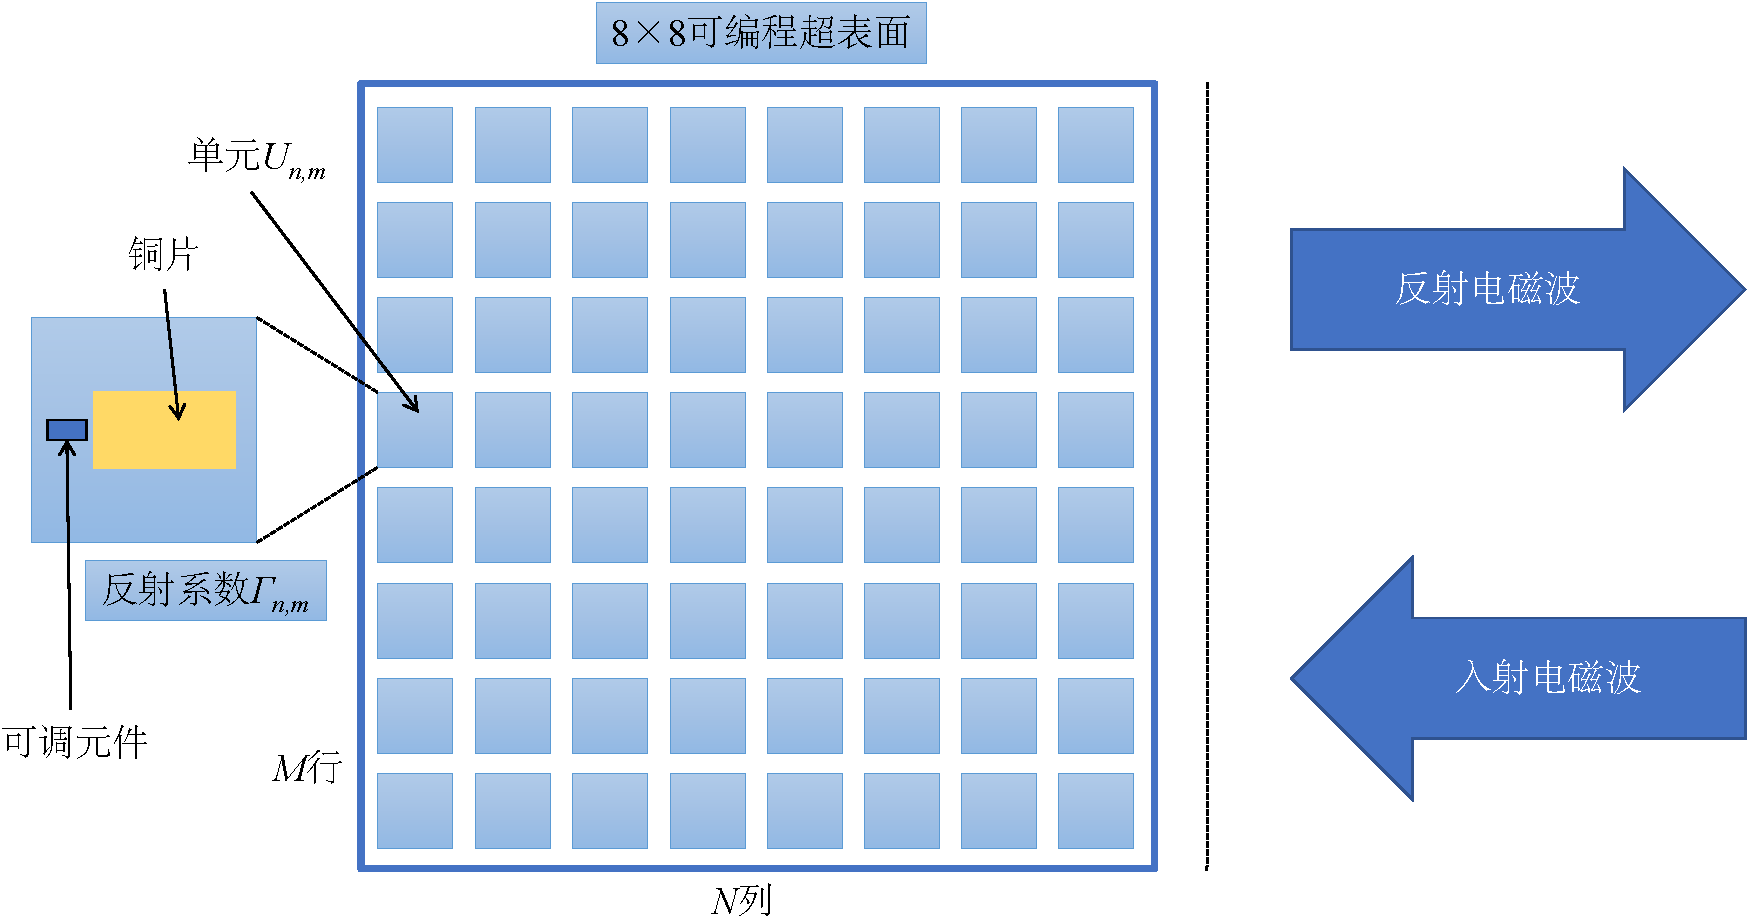
\includegraphics[width=0.8\linewidth]{Figures/ris.pdf}
\end{generalfig}

如\autoref{fig:Reflected-refracted}所示为智能超表面的异常反射、折射示意图,智能超表面可以将入射信号反射和折射到非斯涅尔定律预测的异常方向,可以改变入射电磁波的波形和极化方向\cite{Renzo2019}。
就无线电波的传播而言,基于超材料元表面的RIS就像一个突变的电磁间断,改变了散射场。
如前所述,实现智能超表面的功能的关键要素便是元表面单元结构的设计\cite{5502350, liang2019large}。
元表面是由亚波长金属或电介质散射粒子(称为亚原子)形成的亚波长阵列\cite{basar2019wireless}。
\autoref{fig:Reflected-refracted}描绘了电磁波对于给应的入射角,元表面的预期反射相应和折射相应,与普通平面的反射$ \theta_2 =  \theta_1 $不同,超表面可以使$ \theta_3 \ne \theta_1 $。

\begin{generalfig}[htb]{智能超表面的异常反射、折射}{fig:Reflected-refracted}
	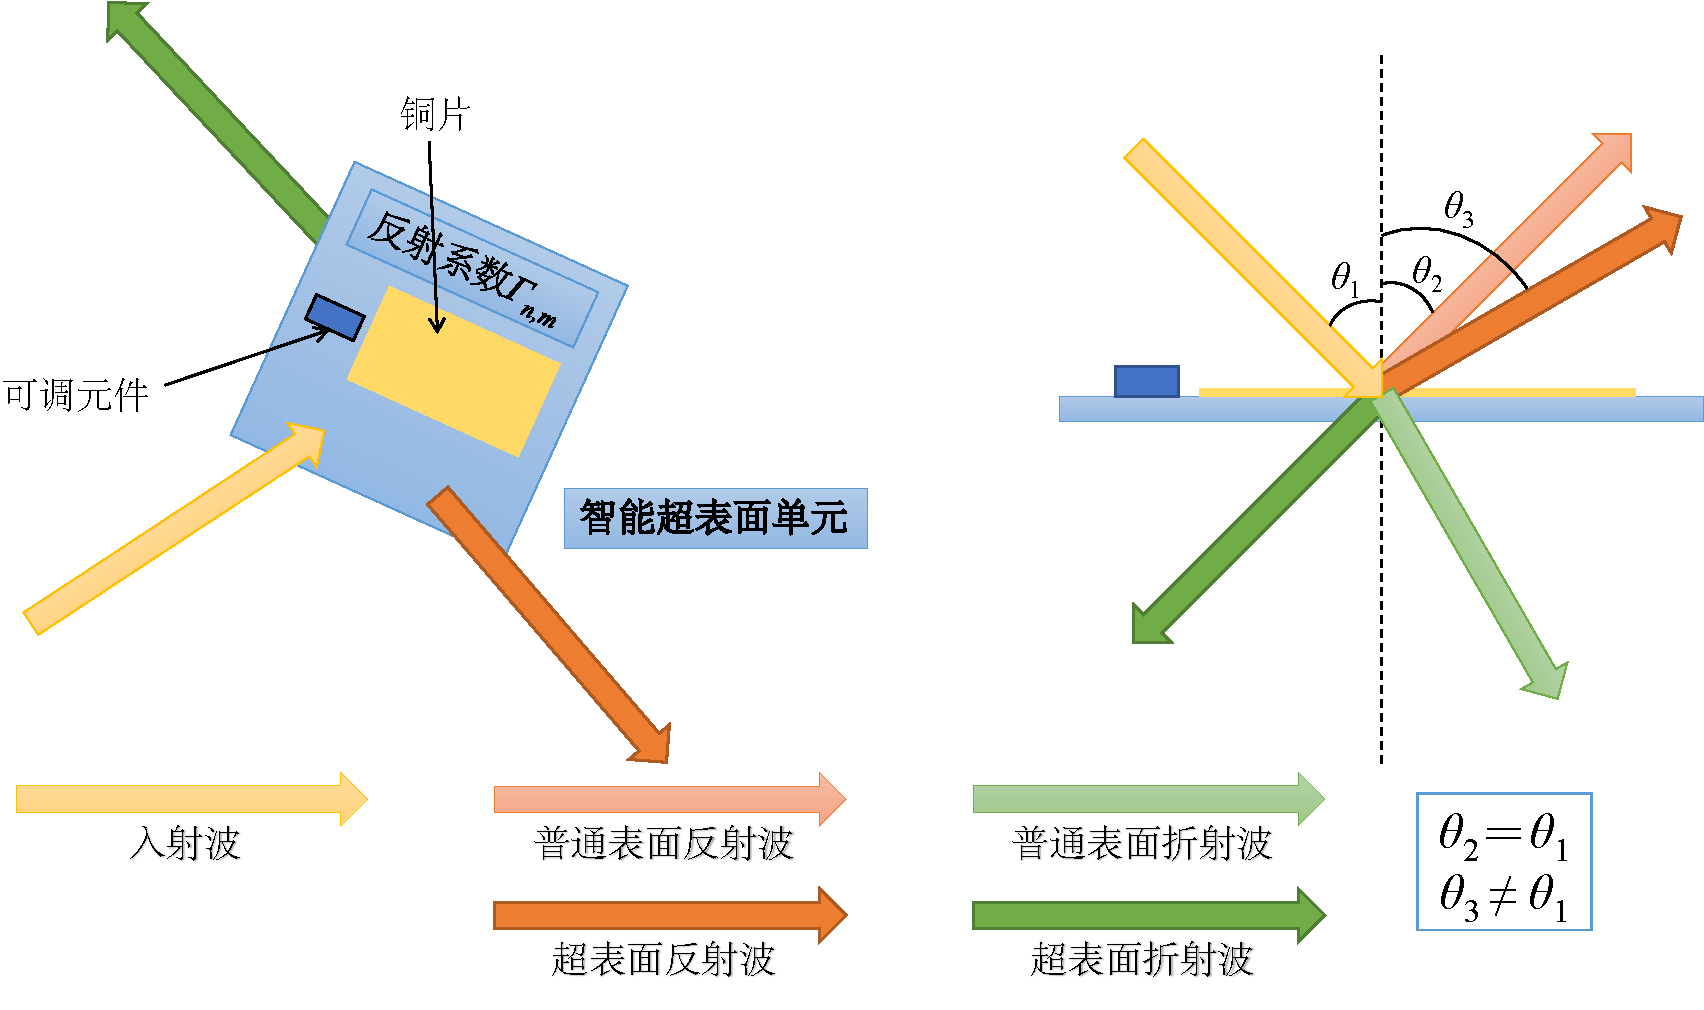
\includegraphics[width=0.8\linewidth]{Figures/Reflected-refracted.pdf}
\end{generalfig}

在智能超表面中,每个单元的反射系数$ \Gamma _ {n,m} $ 是可以根据外界环境调整改变的。
\autoref{fig:ris}上的可调元件一般被安装在单元上。
这样,通过外部的控制电路控制可调元件的状态,就可以操纵元表面上无线电波的波前,以实现信号调制或波束赋形。
智能超表面的中央控制器一般采用现场可编程逻辑门阵列(FPGA)或微控制器(MCU)。
通过软件设计,超表面可以实现对移动通信中电磁信号的实时调控。目前,国内外有关智能超表面在移动通信领域的研究主要集中在两个方向\cite{CHN_zhou2020},下面详细介绍国内外研究现状。

\subsection{国内外现状分析}


目前智能反射面的第一个主要研究方向是利用它进行无线中继,构建智能无线电环境。
如\autoref{fig:Ris-2way}(a)所示,RIS可以被认为是一个多功能的“神奇镜”,将它置于无线通信系统中,可以主动地改善无线传播环境,通过接收机的反馈动态调整反射系数,使得接收机处通过RIS反射和其他路径的叠加信号功率最大化,实现对电磁波资源的“再分配”。
国内外有许多RIS增强系统的主动和被动联合设计的研究:Qingqing Wu等人设计了在单用户和多用户情况下联合的主动和被动波束赋形,可以在接收用户SINR的约束下,最小化总发射功率\cite{Wu2019}。
智能超表面可以使得各个路径的波束在用户(UE)处相干增强,从而最大化接收功率。
Chongwen Huang等人将可重构智能表面用于多用户无线通信,他们通过设计RIS的相移和从基站到用户的功率分配策略,来最大化RIS系统的能效。
此外,文中还介绍了RIS的实际能耗模型。并针对基站发射功率分配和RIS反射系数提出了两个计算效率高的算法。
其中一种采用梯度下降方法设计,而另一种是基于分式规划方法。其中的仿真结果表明,与传统的多天线自动对焦中继相比,该系统能够获得高达300\%的能效\cite{Huang2018a}。

\begin{generalfig}[htb]{智能超表面的两大研究方向}{fig:Ris-2way}
	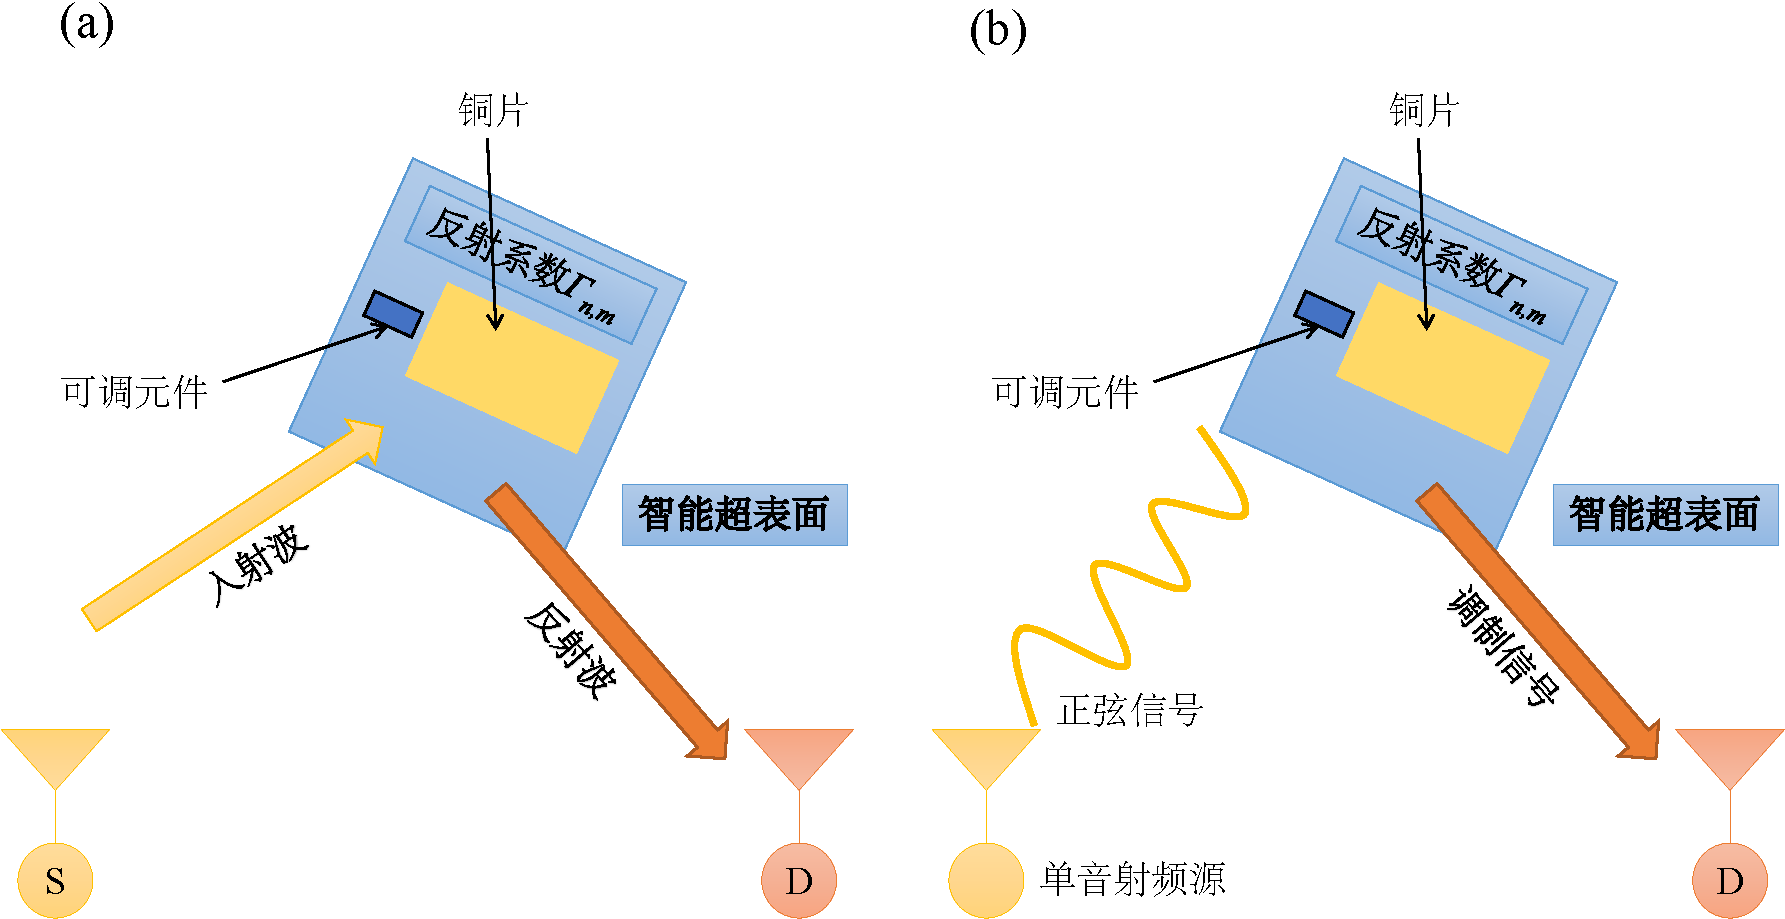
\includegraphics[width=0.8\linewidth]{Figures/Ris-2way.pdf}
\end{generalfig}

绝大多数的研究只停留在理论分析与建模仿真阶段,基于智能超表面的无线通信实验验证系统十分稀缺,目前只有少量的研究:
Zhuqi Li等人在室内环境中部署了一个$ 6 \times 6 $的可重构发射天线阵列,设计了信道分解算法来快速估计无线信道环境\cite{li2019towards}。通过实时配置无线信道,改善通信环境,系统的吞吐量提高到了原来的124\%。
2019年MIT研究团队展示了一个由3000多个无源天线组成的反射面(由几十块PCB板拼接而成),取名为“RFocus”,工作频率为1.6 GHz至3 GHz。
实验表明它可以使接收信号强度平均增加10.5倍,将信道容量平均提升两倍\cite{arun2019rfocus}。
2019年清华大学研究团队最近展示了一个工作在毫米波波段的$ 16 \times 16 $单元的智能超表面。
该RIS每个单元使用四个PIN二极管控制,可实现两比特的反射相位调整。这个系统实现了28.5 GHz下19.1 dBi的天线增益\cite{Dai2020}。

另外一个研究方向是通过智能超表面实现信号的编码与调制。
智能超表面可以灵活地调控电磁信号波前,改变诸如幅度、相位、频率甚至极化方向等电磁参数\cite{CHN_zhou2020}。
这一新型的发射机架构不需要复杂的基带信号处理和高性能的射频链路,未来有希望应用于毫米波通信和Massive MIMO系统中。
其基本结构如\autoref{fig:Ris-2way}(b)所示,基带信号直接作用于智能超表面,通过对反射系数的控制直接调制正弦信号。
东南大学崔铁军院士团队中提出了一种同时在时间和频率上操纵电磁波的时空调制数字可编程超表面,并实现了BFSK调制\cite{zhao2019programmable}。
进一步地,唐万凯等人设计了一个基于可编程表面的正交相移键控(QPSK)无线发射机的原型,实现了2.048 Mbit/s的数据传输速率,视频流也能实时传输\cite{Tang2019Wireless}。

\subsection{本文主要研究内容与组织结构安排}

本文的主要研究内容是如何利用可编程电磁超表面增强5G信号覆盖。
文中首先在\autoref{sec:theory}介绍了电磁超表面的相关基础理论,包括广义反射定律和折射定律以及智能超表面对电磁波的调控机理的理论。

\autoref{sec:modeling}开始对RIS通信系统建模分析,解释了无源金属表面如何散射入射波,然后推导出智能超表面必须如何设计来模拟这种表面,同时控制散射波的方向性,总结了一个严格的路径损耗模型。
并建立智能超表面系统的传输模型,解释了在何种条件下,系统达到最大传输速率。

\autoref{sec:design}设计了一个由可编程超表面及其控制电路构成的智能反射面系统。
从超表面的选择入手,依次介绍了控制电路的设计和驱动、固件的设计。
这章还详细介绍了系统的开发流程,生成了智能超表面系统的控制固件。

\autoref{sec:test}简单地叙述了系统调试方面的内容。
描述了系统组成、系统搭建的过程,重点介绍了FPGA的调试与分析。最后的测试结果表明系统能实现波束调控,达到了设计目的。

最后,在\autoref{sec:conclusion}中总结了本文的研究内容,并对未来的研究工作作了初步分析。

\section{超表面基础理论}\label{sec:theory}

超表面和超材料有着完善复杂的理论,本章根据后续内容的需要着重介绍广义斯涅尔定律和超表面对电磁信号的调控机理。

\subsection{广义反射和折射定律}\label{subsec:snell-law}

电磁波在超表面上会发生相位或幅度的突变,这一现象的理论依据是广义斯涅尔定律\cite{9326394}。
2011年Capasso教授等人发现了相位不连续的电磁波传播,并提出了广义反射和折射定律\cite{yu2011light}。
通过沿着电磁波传播路径,在波长范围内引入突变相移,可以获得控制波前的新自由度。
费马原理指出光线在两点A和B之间的轨迹是最小光程的轨迹,即$ \int_{A}^{B} n(\vec{r}) dr $,其中$ n(\vec{r}) $是局部折射率,由此容易推演得到两种介质之间的反射和折射定律。
在其最普遍的形式中,费马原理可以表述为固定相原理\cite{feynman2010quantum},也就是说,相对于路径的无穷小变化,沿着实际光路累积的相位导数$ \int_{A}^{B} d \varphi (\vec{r}) $将为零。
但是研究表明,通过适当设计两种介质之间的界面,可以在光路中引入波长范围内的突然相移$ \Phi (\vec{r}_\mathrm{s}) $,相移$ \Phi (\vec{r}_\mathrm{s}) $取决于沿界面的坐标$ \vec{r}_\mathrm{s} $。
那么,对于光所走的实际路径,总相移$ \Phi\left(\vec{r}_{\mathrm{s}}\right)+\int_{A}^{B} \vec{k} \cdot d \vec{r} $是固定不变的,其中$ \vec{k} $是传播光的波矢。
这提供了反射和折射定律的一般化,其适用于整个光谱中两种介质之间的大范围的亚波长结构化界面。

\begin{generalfig}[htb]{广义斯涅尔折射定律的示意图}{fig:Snell-Law}
	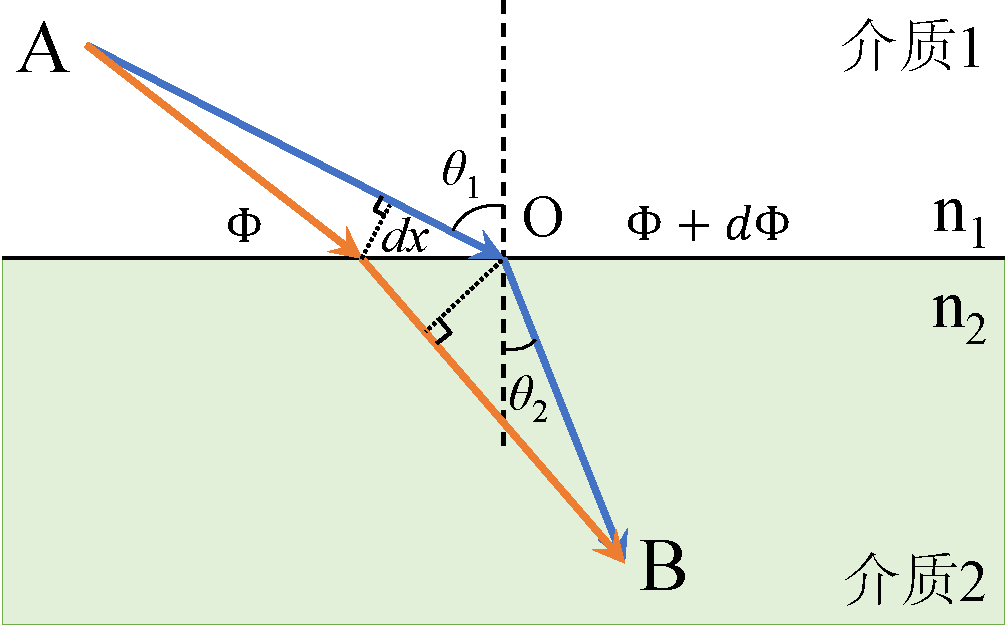
\includegraphics[width=0.5\linewidth]{Figures/Snell-Law.pdf}
\end{generalfig}

下面考虑{\bfseries 广义反射和折射定律},在两种介质的界面上引入一个突变的相移,称为相位不连续,这使得我们可以通过应用费马原理来重新审视反射和折射定律。
\autoref{fig:Snell-Law}中的入射平面波入射角为$\theta_1$,假设两条光路无限接近实际光路,那么它们之间的相位差为零,有:
\begin{equation}
	k_\mathrm{o} n_1 \sin (\theta_1) dx + (\Phi + d\Phi) = k_\mathrm{o} n_2 \sin (\theta_2) dx + \Phi
	\label{eq:Generalized-snell-law-pre}
\end{equation}
其中$ \theta_2 $为折射角,$ \Phi $和$ \Phi + d\Phi $分别是两条路径穿过界面位置处的相位不连续性,$ dx $是两条路径界面处的距离差,$n_1$是上层介质的折射率,$n_2$为下层介质的折射率,$k_\mathrm{o}=2 \pi / \lambda_\mathrm{o}$,$\lambda_\mathrm{o}$为真空中的光波波长。

如果沿界面的相位梯度被设计为常数,由\autoref{eq:Generalized-snell-law-pre}可以推导出广义的斯涅尔折射定律:
\begin{equation}
	n_2 \sin \theta_2 - n_1 \sin \theta_1 = \frac{1}{k_\mathrm{o}} \frac{d \Phi}{dx}
	\label{eq:Generalized-snell-law}
\end{equation}
\autoref{eq:Generalized-snell-law}意味着折射光束可以具有任意方向,只要沿界面引入相位不连续性的合适的恒定梯度$d\Phi/dx$。
由于在\autoref{eq:Generalized-snell-law}中引入了非零的相位梯度$d\Phi/dx$,两个入射角$\pm \theta_1$会导致不同的折射角。
因此,全内反射在$n_2<n_1$时有两种可能的临界角:
\begin{equation}
	\theta_{\mathrm{c}}=\arcsin \left(\pm \frac{n_{2}}{n_{1}}-\frac{\lambda_{\mathrm{o}}}{2 \pi n_{1}} \frac{d \Phi}{d x}\right)
\end{equation}

同理,由\autoref{eq:Generalized-snell-law}也可以推导出广义斯涅尔反射定律。对于反射的情况,入射波和反射波都在介质1中,所以有$n_2=n_1$,可得:
\begin{equation}
	\sin \theta_2 - \sin \theta_1 = \frac{1}{k_\mathrm{o} n_1} \frac{d \Phi}{dx}
	\label{eq:Generalized-snell-law-reflection}
\end{equation}
此时$\theta_2$是反射角,入射角$\theta_1$和反射角$\theta_2$之间存在非线性关系,这与传统的镜面反射明显不同。
由\autoref{eq:Generalized-snell-law-reflection}可知总有一个临界角$\theta_{\mathrm{c}}^{\prime}$满足:
\begin{equation}
	\theta_{\mathrm{c}}^{\prime}=\arcsin \left(1-\frac{\lambda_{\mathrm{o}}}{2 \pi n_{1}}\left|\frac{d \Phi}{d x}\right|\right)
\end{equation}
在入射角$\theta_1 = \theta_{\mathrm{c}}^{\prime}$时,反射波束将不存在。

广义反射和折射定律可以统一写成如下的形式\cite{ding2017gradient}:
\begin{eqnarray}
	k_{x}^{(r)}-k_{x}^{(i)}=\frac{d \Phi}{d x} \\
	k_{x}^{(t)}-k_{x}^{(i)}=\frac{d \Phi}{d x}
\end{eqnarray}
其中$k_{x}^{(i, r, t)}=k_{\mathrm{o}} n_{i, i, t} \sin \theta_{i, r, t}$表示平面波矢量。标号$i$表示入射侧的参量,标号$r$表示反射侧的参量,标号$t$表示折射侧的参量。
当$\frac{d \Phi}{d x}=0$时,即得到经典的斯涅尔定律。

广义斯涅尔定律为超表面的设计提供了理论指导,在设计超表面的过程中,我们只需要将它分解为二维亚波长单元,分析每个单元对电磁波带来的附加相位,通过对反射阵列的附加相位的设计,结合波束赋形理论,就可以实现对电磁波的灵活调控。

\subsection{超表面对电磁波的调控机理}

文献\normalcite{Chen2018dian}中研究了透射式智能超表面对电磁波的调控机理。
本小节基于此,推导出反射式超表面对电磁波的调控机理。
我们知道,智能超表面是通过在分界面处引入一个附加相位来实现对电磁波的调控,从而引起等相位面的改变。

超表面的反射单元通过有序的周期性排列组成,通过设定各个单元的反射系数可以实现对电磁波波束的灵活调控。
下面将通过把球面波调控为平面波并向垂直与阵面方向反射的例子介绍超表面对电磁波的调控机理。
如\autoref{fig:ris}所示,图中每个矩形贴片代表电磁超表面的一个结构单元,一共有$M \times N$个结构单元。
\autoref{fig:phase}中为相位补偿示意图,其中,$F(m,n)$代表馈源的相位中心到超表面结构单元$(m,n)$的相位延迟,$S(m,n)$表示超表面单元$(m,n)$上入射波与反射波的相位差。
根据上述参数,反射波的相位分布可表示为:
\begin{equation}
	\left\{
		\begin{array}{l}
			\varphi(m,n)=F(m,n)+S(m,n) \\
			\varphi(0,0)=F(0,0)+S(0,0)
		\end{array}
	\right.
\end{equation}
其中,$\varphi(m,n)$与$\varphi(0,0)$分别代表了结构单元$(m,n)$与$(0,0)$的反射波的出射相位。
 
\begin{generalfig}[htb]{相位补偿示意图}{fig:phase}
	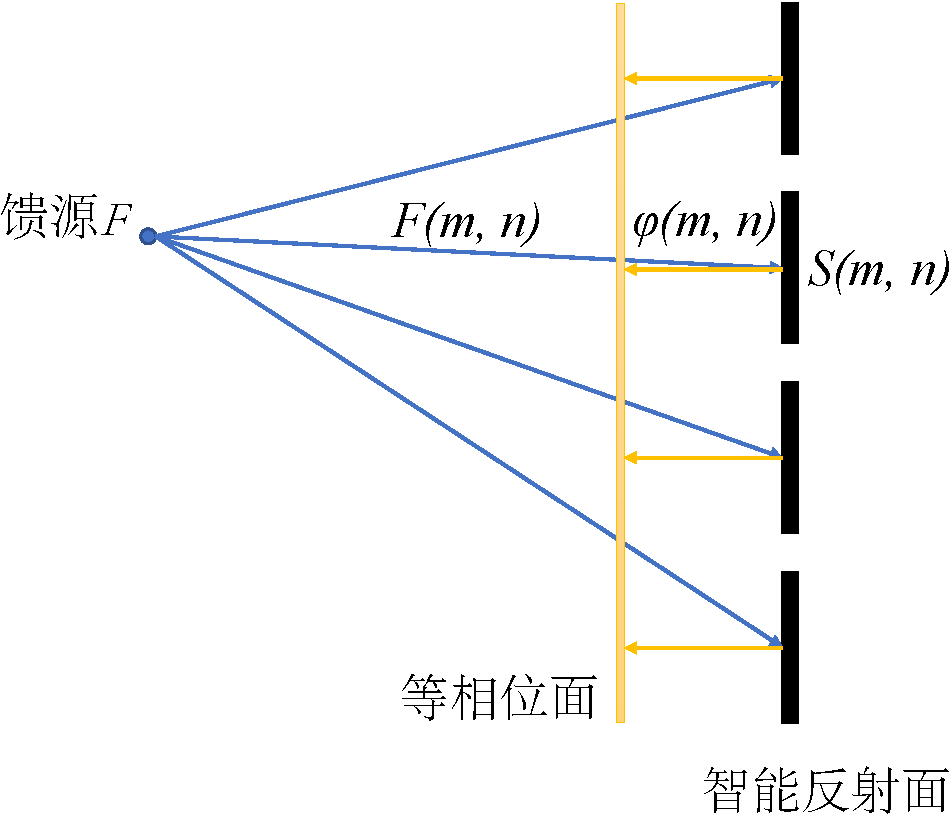
\includegraphics[width=0.5\linewidth]{Figures/phase.pdf}
\end{generalfig}

设计目的是垂直反射,为了形成平行于超表面的等相位面,出射相位之间需要满足以下关系式:
\begin{equation}
	\varphi (m,n) - \varphi (0,0) = 2p \pi, \; p = 0, \pm 1,\pm 2,\dots 
\end{equation}
联立上述两式,可以得到:
\begin{equation}
	S(m,n)-S(0,0)=-F(m,n)+F(0,0)+2p\pi, \; p = 0, \pm 1,\pm 2,\dots 
\end{equation}
其中,$S(0,0)$是参考相位,它的值应根据应用时的具体需求去选择,$S(0,0)$确定之后,可推出$S(m,n)$。

当然,反射后的波束方向不会局限于垂直阵面表面,可以根据应用需要任意选择。
如果希望反射后电磁波波束在$(\theta_0,\phi_0)$方向上,那么位于$(m,n)$位置上的结构单元相对结构单元$(0,0)$的相位差可表示为:
\begin{equation}
	\varphi(m,n)-\varphi(0,0)=k(md\sin⁡\theta_0 \cos⁡\phi_0+nd\sin⁡\theta_0 \sin\phi_0)+2p\pi,\;p = 0, \pm 1,\dots 
\end{equation}
其中,$k$为波数,$k=2\pi/ \lambda$,$\lambda$为波长,$d$为单元间距。要使反射后电磁波波束在$(\theta_0,\phi_0)$方向,那么$(\theta_0,\phi_0)$方向应形成等相位面。
此时,由阵列理论可知,超表面上反射波与入射波的相位差$S(m,n)$应满足:
\begin{equation}
	\begin{aligned}
		S(m,n)&=-F(m,n)-(\varphi(m,n)-\varphi(0,0))+2p\pi \\
	          &=-F(m,n)-k(md\sin⁡\theta_0 \cos⁡\phi_0+nd\sin⁡\theta_0 \sin\phi_0)+2p\pi ,\\
			  &\qquad \qquad \qquad \qquad \qquad \qquad \qquad \qquad \qquad p = 0, \pm 1,\dots 
	\end{aligned}
\end{equation}
根据上式,只要反射波波束方向$(\theta_0,\phi_0)$确定,发射机相位中心到超表面结构单元$(m,n)$的相位延迟$F(m,n)$确定,就可以确定超表面上所需要的反射相位关系$S(m,n)$。之后,只要将超表面阵列中各个结构单元的反射相位关系与超表面结构参数意义对应。
通过控制表面单元的电压或者表面元件的通断,便可以完成能够将馈源发射的电磁波反射到特定方向的电磁超表面的设计,实现对电磁波的灵活调控。

\subsection{本章小结}

本章主要介绍了广义斯涅尔定律和超表面对电磁信号的调控机理,为后面的理论研究和系统实现打下了基础。

\section{物理、传播和路径损耗建模}\label{sec:modeling}

本章中,我们使用物理光学知识导出了远场路径损耗\cite{emil2019intelligent},并解释了为什么智能超表面由许多元素组成,这些元素单独充当散射体,但可以在特定波束宽度的期望方向上联合波束赋形。本章首先将从无源金属表面的散射分析引入。

\subsection{无源金属表面}\label{subsec:metal-plate}

在这一节中,我们总结了由有限尺寸的无源的完全导电的金属板散射的波形的场强和波束宽度的研究。这些结果将被用来解释智能超表面的理想工作状态。

我们考虑一个尺寸为$a \times b$的厚度可以忽略的矩形完美导电板,且位于水平面上(即$\boldsymbol{e}_{x}, \boldsymbol{e}_{y}$所在平面)。一个距离为$d_i$的很远的点源辐射具有波数为$k$($k = 2\pi / \lambda$,$\lambda$为波长)的线性极化电磁波。
为了便于讨论,我们假设源的极化是这样的,即电场平行于$\boldsymbol{e}_{x}$,而磁场位于$\boldsymbol{e}_{y}, \boldsymbol{e}_{z}$所跨越的平面上。
$\theta_{i} \in\left[0, \frac{\pi}{2}\right]$表示为入射角,即电磁波的坡印亭矢量与$\boldsymbol{e}_{z}$的夹角,$\theta_{s}$为散射角,如\autoref{fig:metal-plate}所示。

\begin{generalfig}[htb]{入射波被金属板散射示意图}{fig:metal-plate}
	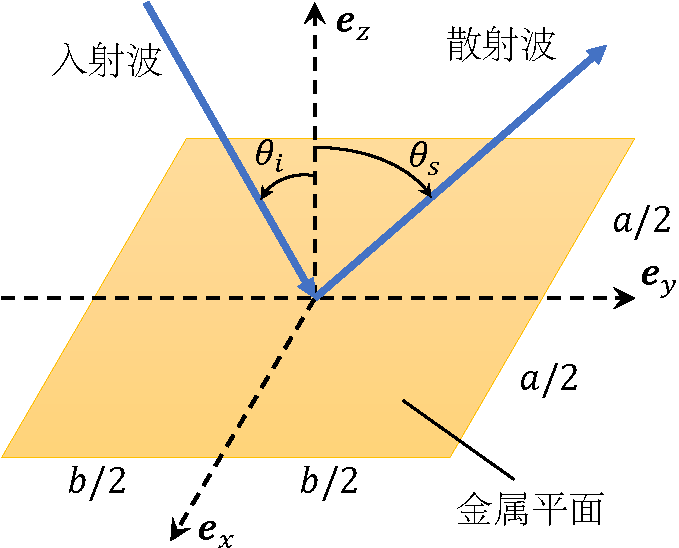
\includegraphics[width=0.5\linewidth]{Figures/metal-plate.pdf}
\end{generalfig}

进一步假设,相对于金属板的尺寸,$d_i$足够大,符合远场模型。此时入射波为幅度为$E_i$的平面波。
这时入射的平面波的电场和磁场分布可以表示为:
\begin{equation}
	\begin{array}{l}
		\mathbf{E}_{i}=E_{i} e^{-j k\left(\sin \left(\theta_{i}\right) y-\cos \left(\theta_{i}\right) z\right)} \boldsymbol{e}_{x} \\
		\mathbf{H}_{i}=-\frac{E_{i}}{\eta}\left(\cos \left(\theta_{i}\right) \boldsymbol{e}_{y}+\sin \left(\theta_{i}\right) \boldsymbol{e}_{z}\right) e^{-j k\left(\sin \left(\theta_{i}\right) y-\cos \left(\theta_{i}\right) z\right)}
	\end{array}
	\label{eq:e-field}
\end{equation}
其中$\eta$是介质的特征阻抗。

电场会引起电子在金属板中的运动。
由于电场与$\boldsymbol{e}_{y}$正交,电子将沿$\boldsymbol{e}_{x}$方向移动,而不会沿$\boldsymbol{e}_{y}$方向移动。
因为金属板的厚度忽略不计,电子也不会沿$\boldsymbol{e}_{z}$方向移动。
运动的电子感应电磁辐射,产生散射波。

\begin{lemma}
	\label{lemma:scattered-field}
	在$\boldsymbol{e}_{y}, \boldsymbol{e}_{z}$平面内,对于任意观察角度$\theta_{s} \in\left[0, \frac{\pi}{2}\right]$(相对于$\boldsymbol{e}_{z}$),在远场观察距离$r \geq \frac{2 \max \left(a^{2}, b^{2}\right)}{\lambda}$时,散射场的平方幅度为:
	\begin{equation}
		S\left(r, \theta_{s}\right)=\left(\frac{a b}{\lambda}\right)^{2} \frac{E_{i}^{2}}{r^{2}} \cos ^{2}\left(\theta_{i}\right)\left(\frac{\sin \left(\frac{\pi b}{\lambda}\left(\sin \left(\theta_{s}\right)-\sin \left(\theta_{i}\right)\right)\right)}{\frac{\pi b}{\lambda}\left(\sin \left(\theta_{s}\right)-\sin \left(\theta_{i}\right)\right)}\right)^{2}
		\label{eq:scattered-field}
	\end{equation}
\end{lemma}

\begin{proof}
	这个结果来自标准的物理光学技术(忽略边缘效应)\cite{balanis2012advanced}。
\end{proof}

从\autoref{eq:scattered-field}中关于散射场的平方幅度的公式可以发现,对于我们考虑的极化方式来说,当观察角度$\theta_{s}=\theta_{i}$即镜面反射时,$S\left(r, \theta_{s}\right)$达到最大值,这和斯涅尔反射定律所描述的是吻合的。

\subsubsection{散射波的波束宽度}

\autoref{eq:scattered-field}揭示了散射场就像是一个波束,随着$\theta_{s}$远离$\theta_{i}$,强度越来越弱。在\normalcite{emil2019intelligent}中,作者运用三角函数和泰勒展开的数学知识推导出散射波的$-3\,\mathrm{dB}$宽度为:
\begin{equation}
	2\left|\theta_{s}-\theta_{i}\right|<2\sqrt{\frac{1}{2} \frac{3 \lambda^{2}}{\pi^{2} b^{2} \cos ^{2}\left(\theta_{i}\right)}}=2\sqrt{\frac{3}{2}} \frac{\lambda}{\pi b \cos \left(\theta_{i}\right)}
\end{equation}

这个不等式表明,$-3\,\mathrm{dB}$的波束宽度与金属板板宽$b$成反比。波束宽度也与波长$\lambda$成正比,因此普通尺寸的板可以在可见光谱中提供非常窄的波束宽度,就像一束光照射在镜子上一样。
但是在典型的无线电光谱波段中,波束宽度要宽四至五个数量级。

\subsubsection{多个相邻金属表面}

由于单个金属板的尺寸有限,有时可以部署多个相邻的板。
如果板子之间的间隙足够大,那么耦合效应可以忽略。
当来自不同的金属板的散射场在给定位置被接收时,相对的相移将导致干涉相长或干涉相消。
在理想的干涉相长下,来自$N$个平板的平方场强为:
\begin{equation}
	\left(N \sqrt{S\left(r, \theta_{s}\right)}\right)^{2}=N^{2} S\left(r, \theta_{s}\right)
	\label{eq:Multiple-Metallic-Surfaces}
\end{equation}

\autoref{eq:Multiple-Metallic-Surfaces}表明,只要总面积确定,无论是由许多小的还是几个大的金属板组成,最大接收功率是相同的。

\subsection{智能超表面的系统模型}

智能超表面的主要目的是实现“异常反射”\cite{liang2015anomalous},这意味着对散射场进行整形,使主波束指向接收器。考虑一个由与\autoref{fig:metal-plate}相同尺寸的超表面和相同的撞击平面波组成的反射系统。RIS的目标是实现全反射,并将主光束指向我期望方向$\theta_r$。
因此,超表面必须被设计成获得反射或散射波的以下理想场分布:
\begin{equation}
	\begin{array}{l}
		\mathbf{E}_{r}=E_{r} e^{-j k\left(\sin \left(\theta_{r}\right) y+\cos \left(\theta_{r}\right) z\right)} \boldsymbol{e}_{x} \\
		\mathbf{H}_{r}=-\frac{E_{r}}{\eta}\left(\sin \left(\theta_{r}\right) \boldsymbol{e}_{z}-\cos \left(\theta_{r}\right) \boldsymbol{e}_{y}\right) e^{-j k\left(\sin \left(\theta_{r}\right) y+\cos \left(\theta_{r}\right) z\right)}
	\end{array}
\end{equation}

使用\autoref{subsec:snell-law}中介绍的广义斯涅尔定律,利用\autoref{eq:Generalized-snell-law-reflection},可以通过调整超表面相位分布或表面阻抗将入射波$\left(\mathbf{E}_{i}, \mathbf{H}_{i}\right)$转换成散射波$\left(\mathbf{E}_{r}, \mathbf{H}_{r}\right)$。
在超表面上$(z = 0)$,入射和反射电场的叠加可以写成\cite{Asadchy_2016}:
\begin{equation}
	\mathbf{E}_{t}=E_{i} e^{-j k \sin \left(\theta_{i}\right) y} \boldsymbol{e}_{x}+E_{r} e^{-j k \sin \left(\theta_{r}\right) y} \boldsymbol{e}_{x}
\end{equation}
由此可得,期望反射系数的期望相位是:
\begin{equation}
	\phi_{r}(y)=\angle\left(\frac{E_{r} e^{-j k \sin \left(\theta_{r}\right) y}}{E_{i} e^{-j k \sin \left(\theta_{i}\right) y}}\right)=-k \sin \left(\theta_{r}\right) y+k \sin \left(\theta_{i}\right) y
\end{equation}
并且对$y$进行微分给出了广义斯内尔定律中反射系数的梯度:
\begin{equation}
	k\left(\sin \left(\theta_{i}\right)-\sin \left(\theta_{r}\right)\right)=\frac{d \phi_{r}(y)}{d y}
\end{equation}
它给出了$\theta_i,\theta_r$和局部表面相位$\phi_{r}(y)$之间的关系。

\subsubsection{传播和路径损耗模型}

与单纯的金属表面不同,智能超表面必须由许多小单元组成,细致的配置每个单元的相位,可以获得角度为$\theta_r$的主反射波束。
如\autoref{subsec:metal-plate}中所述,\autoref{eq:e-field}中的入射波电场在$\boldsymbol{e}_{x}$方向上感应出表面电流。
通过调整每个元件的表面阻抗,调整该电流,以获得近似广义斯内尔定律所需的表面相位分布。

\begin{lemma}
	当使用智能超表面向$\theta_r$方向反射信号时,任意观察角度$\theta_{s} \in\left[-\frac{\pi}{2}, \frac{\pi}{2}\right]$下,在远场观察距离$r \geq \frac{2 \max \left(a^{2}, b^{2}\right)}{\lambda}$时,散射场平方幅度为:
	\begin{equation}
		S_{\mathrm{IRS}}\left(r, \theta_{s}, E_{i}^{2}\right) =\left(\frac{a b}{\lambda}\right)^{2} \frac{E_{i}^{2} \cos ^{2}\left(\theta_{i}\right)}{r^{2}}\left(\frac{\sin \left(\frac{\pi b}{\lambda}\left(\sin \left(\theta_{s}\right)-\sin \left(\theta_{r}\right)\right)\right)}{\frac{\pi b}{\lambda}\left(\sin \left(\theta_{s}\right)-\sin \left(\theta_{r}\right)\right)}\right)^{2}
	\end{equation}
\end{lemma}

\begin{proof}
	超表面的厚度可以忽略不计,这使得我们可以写出超表面上某处$(z=0, y=y^\prime)$的电流密度$J_{x}=\frac{2 E_{i}}{\eta} \cos \left(\theta_{i}\right) e^{-j k \sin \left(\theta_{r}\right) y^{\prime}}$。假设超表面是无损的,上述引理利用引理~\ref{lemma:scattered-field}可以证明。
\end{proof}

假设基站端的发射机发射功率为$P_t$,发射天线的增益为$G_t$,$E_i$和$P_t$之间的关系可以表示为:
\begin{equation}
	\frac{E_{i}^{2}}{2 \eta}=\frac{P_{t} G_{t}}{4 \pi d_{i}^{2}}
\end{equation}
此外,假设接收器天线的有效面积为$\frac{\lambda^2}{4\pi} G_r$,其中$G_r$为接收天线的增益。可得,距离为$r$时,在方向$\theta_r$上,接收信号功率$P_r$为:
\begin{equation}
	P_{r}\left(P_{t}, d_{i}, r, \theta_{s}\right)=\frac{1}{2 \eta} S_{\mathrm{IRS}}\left(r, \theta_{s}, \frac{P_{t} G_{t} \eta}{2 \pi d_{i}^{2}}\right)\left(\frac{\lambda^{2}}{4 \pi} G_{r}\right)
\end{equation}

\begin{corollary}
	当使用智能超表面向$\theta_r$方向上反射电磁波时,远场距离为$r$时的路径损耗是:
	\begin{equation}
		\begin{array}{l}
			\beta_{\mathrm{IRS}}\left(r, d_{i}, \theta_{s}\right)=\frac{P_{r}\left(P_{t}, d_{i}, r, \theta_{s}\right)}{P_{t}} \\
			=\frac{G_{t} G_{r}}{(4 \pi)^{2}}\left(\frac{a b}{d_{i} r}\right)^{2} \cos ^{2}\left(\theta_{i}\right)\left(\frac{\sin \left(\frac{\pi b}{\lambda}\left(\sin \left(\theta_{s}\right)-\sin \left(\theta_{r}\right)\right)\right)}{\frac{\pi b}{\lambda}\left(\sin \left(\theta_{s}\right)-\sin \left(\theta_{r}\right)\right)}\right)^{2}
		\end{array}
	\end{equation}

	当接收机处于理想位置时,即$\theta_s=\theta_r$,路径损耗简化为:
	\begin{equation}
		\beta_{\mathrm{IRS}}\left(r, d_{i}, \theta_{r}\right)=\frac{G_{t} G_{r}}{(4 \pi)^{2}}\left(\frac{a b}{d_{i} r}\right)^{2} \cos ^{2}\left(\theta_{i}\right)
	\end{equation}
\end{corollary}

\subsubsection{智能超表面的散射体阵列模型}

如上所述,大小为$a \times b$的智能超表面由许多小于$\lambda$的表面元素组成,假设每个单元的大小为$\frac{a}{N_a} \times \frac{b}{N_b}$。则发射机和接收机通过第$n$个单元的路径损耗可以表述为:
\begin{equation}
	\beta_{\mathrm{IRS}}^{s}\left(r, d_{i}, \theta_{r}\right)=\frac{G_{t} G_{r}}{(4 \pi)^{2}}\left(\frac{a b}{N_{a} N_{b} d_{i} r}\right)^{2} \cos ^{2}\left(\theta_{i}\right)
\end{equation}
由于假设的是远场的情况,所以$\beta_{\mathrm{IRS}}^{s}\left(r, d_{i}, \theta_{r}\right)$对所有单元来说都是一样的。
根据\autoref{eq:Multiple-Metallic-Surfaces},如果所有$N=N_a N_b$个单元相干增强,则发射机和接收机之间通过整个智能超表面的路径损耗为:
\begin{equation}
	\left(N \sqrt{\beta_{\mathrm{IRS}}^{s}\left(r, d_{i}, \theta_{r}\right)}\right)^{2}=\beta_{\mathrm{IRS}}\left(r, d_{i}, \theta_{s}\right)
\end{equation}
因此,我们可以将智能超表面解释为一组特殊的散射体。这些散射体在接收器处对其反射信号进行相位校准,实现相干增强,从而实现“异常”反射。

\subsection{智能超表面的传输模型}\label{subsec:transmission}

\subsubsection{单输入单输出(SISO)信道}

考虑从单天线源到单天线目的地的通信(SISO)。确定性平坦衰落信道表示为$h_{\mathrm{sd}} \in \mathbb{C}$,目的地接收到的信号是:
\begin{equation}
	y=h_{\mathrm{sd}} \sqrt{p} s + n
\end{equation}
其中$p$是发射功率,$s$是单位功率信息信号,$n \sim \mathcal{N}_{\mathbb{C}}\left(0, \sigma^{2}\right)$是接收机噪声。为了便于分析,天线增益包含在信道中。
该单输入单输出(SISO)信道的容量为:
\begin{equation}
	R_{\mathrm{SISO}}=\log _{2}\left(1+\frac{p\left|h_{\mathrm{sd}}\right|^{2}}{\sigma^{2}}\right)
\end{equation}
通过在通信中加入额外的设备,可以潜在地增加容量。

\subsubsection{智能超表面使能的传输}

下面考虑智能超表面使能的传输,智能超表面被配置为使反射波束指向目的地。
因为它不能获取信道状态信息(Channel State Information, CSI),
假设智能超表面辅助增强通信具有确定性平坦衰落的信道。

\begin{generalfig}[htb]{智能超表面使能的传输示意图}{fig:RIS-transmission}
	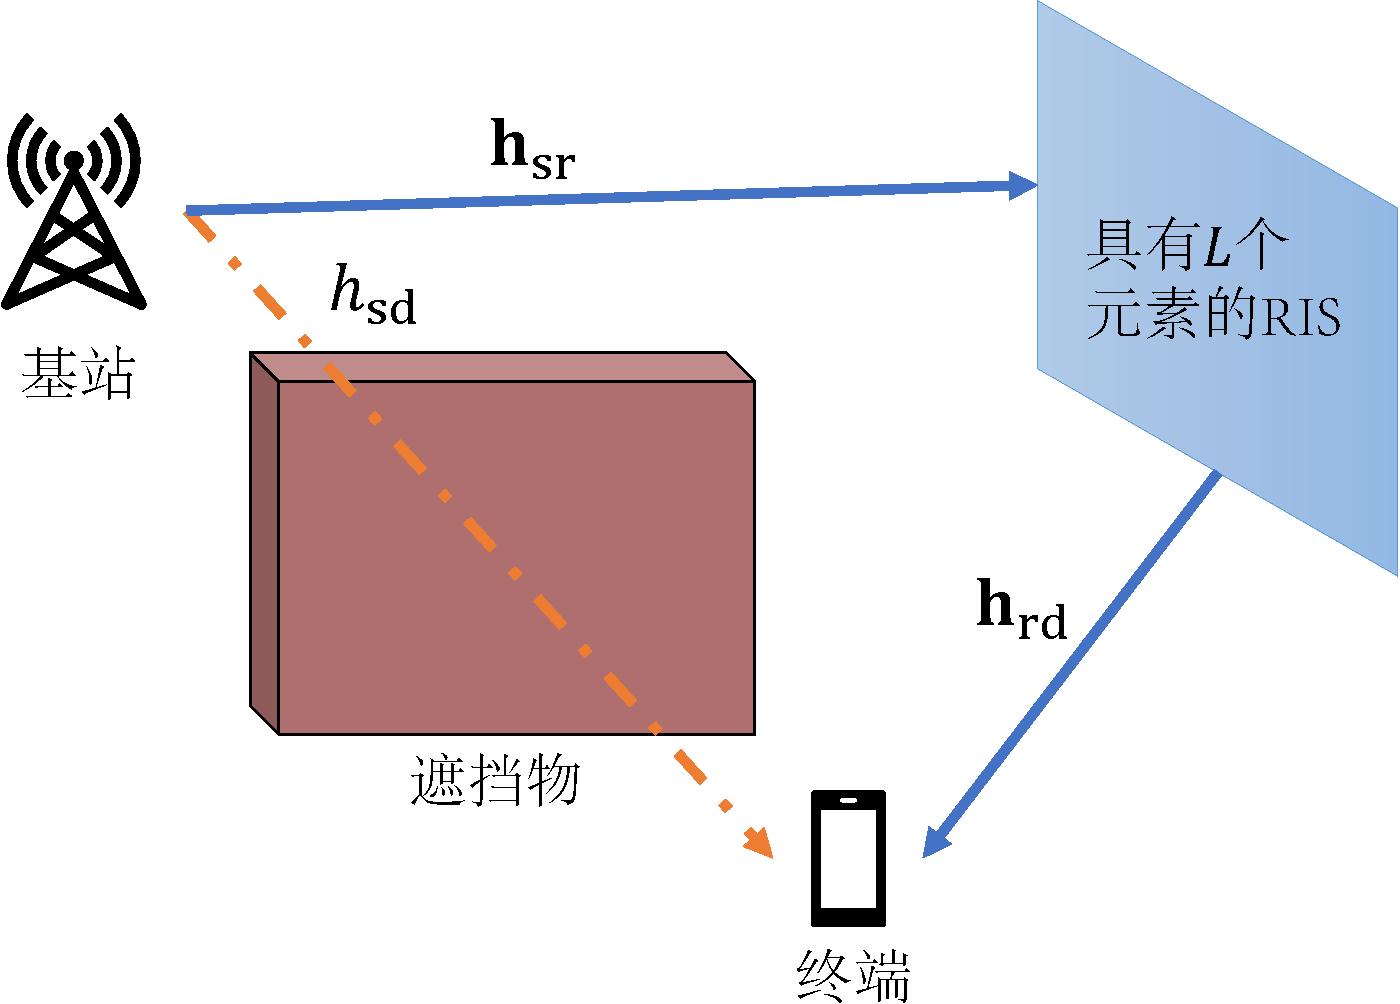
\includegraphics[width=0.6\linewidth]{Figures/RIS-transmission.pdf}
\end{generalfig}

如\autoref{fig:RIS-transmission}所示,RIS由总共由$L$个元素组成。从基站到智能超表面的确定性信道表示为$\mathbf{h}_{\mathrm{sr}} \in \mathbb{C}^{L}$,$\left[\mathbf{h}_{\mathrm{sr}}\right]_{l}$代表第$l$个结构单元的信道。从智能超表面到终端的信道表示为$\mathbf{h}_{\mathrm{rd}} \in \mathbb{C}^{L}$,每个单元的尺寸都小于入射波波长,这样可以认为它以近似恒定的增益向所有感兴趣的方向散射输入信号\cite{emil2019intelligent}。
智能超表面的所有单元的反射系数可以表示为:
\begin{equation}
	\boldsymbol{\Theta}=\alpha \operatorname{diag}\left(e^{j \theta_{1}}, \ldots, e^{j \theta_{L}}\right)
\end{equation}
其中$\alpha \in (0,1]$是固定振幅反射系数,$\theta_{1}, \ldots, \theta_{L}$是RIS单元的相移变量,接收端的信号可以表示为:
\begin{equation}
	y=\left(h_{\mathrm{sd}}+\mathbf{h}_{\mathrm{sr}}^{\mathrm{T}} \boldsymbol{\Theta} \mathbf{h}_{\mathrm{rd}}\right) \sqrt{p} s+n
\end{equation}
其中$p$、$s$和$n$的定义与SISO情况相同。

\begin{lemma}
	智能超表面使能的网络的信道容量为:
	\begin{align}
		R_{\mathrm{IRS}}(L) &=\max _{\theta_{1}, \ldots, \theta_{L}} \log _{2}\left(1+\frac{p\left|h_{\mathrm{sd}}+\mathbf{h}_{\mathrm{sr}}^{\mathrm{T}} \boldsymbol{\Theta} \mathbf{h}_{\mathrm{rd}}\right|^{2}}{\sigma^{2}}\right) \label{eq:R-RIS1} \\
		&=\log _{2}\left(1+\frac{p\left(\left|h_{\mathrm{sd}}\right|+\alpha \sum_{l=1}^{L}\left|\left[\mathbf{h}_{\mathrm{sr}}\right]_{l}\left[\mathbf{h}_{\mathrm{rd}}\right]_{l}\right|\right)^{2}}{\sigma^{2}}\right)
	\end{align}
\end{lemma}

\begin{proof}
	对于任意给定的$\boldsymbol{\Theta}$,\autoref{eq:R-RIS1}中的速率表达式是由加性白高斯噪声信道的容量获得的。注意$ \mathbf{h}_{\mathrm{sr}}^{\mathrm{T}} \boldsymbol{\Theta} \mathbf{h}_{\mathrm{rd}} = \alpha \sum_{l=1}^{L} e^{j\theta_l} \left[\mathbf{h}_{\mathrm{sr}}\right]_{l}\left[\mathbf{h}_{\mathrm{rd}}\right]_{l} $。当单元的相移$\theta_{l}=\arg \left(h_{\mathrm{sd}}\right)-\arg \left(\left[\mathbf{h}_{\mathrm{sr}}\right]_{n}\left[\mathbf{l}_{\mathrm{rd}}\right]_{l}\right)$时,系统达到最大传输速率。
\end{proof}

\subsection{本章小结}

在本章中,我们首先在解释了无源金属表面如何散射入射波,然后推导出智能超表面必须如何设计来模拟这种表面,同时控制散射波的方向性,总结了一个严格的路径损耗模型。
并建立智能超表面系统的传输模型,解释了在何种条件下,系统达到最大传输速率。
下一章将详细叙述智能超表面系统的设计与实现。

\section{系统设计与实现}\label{sec:design}

\subsection{智能超表面选择}\label{subsec:28-GHz-RIS}

本设计选用了\autoref{fig:28-GHz-RIS}所示的工作频点为28 GHz的智能超表面。
其中\autoref{fig:28-GHz-RIS}(a)为三维仿真图,\autoref{fig:28-GHz-RIS}(b)为实物正视图,\autoref{fig:28-GHz-RIS}(c)为实物立体图。

\begin{figure}[htb]
	\centering
	\subfloat[三维仿真图]{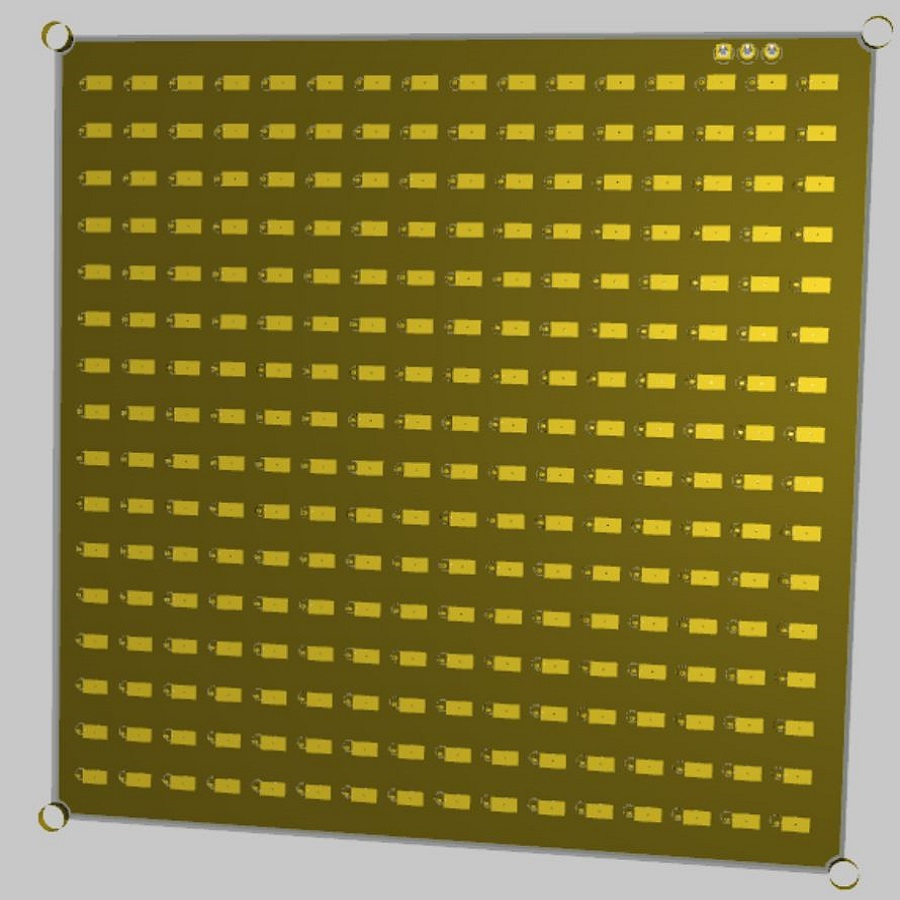
\includegraphics[width=0.3\linewidth]{Figures/28-GHz-RIS-3D.JPG}}
	\hfil
	\subfloat[实物正视图]{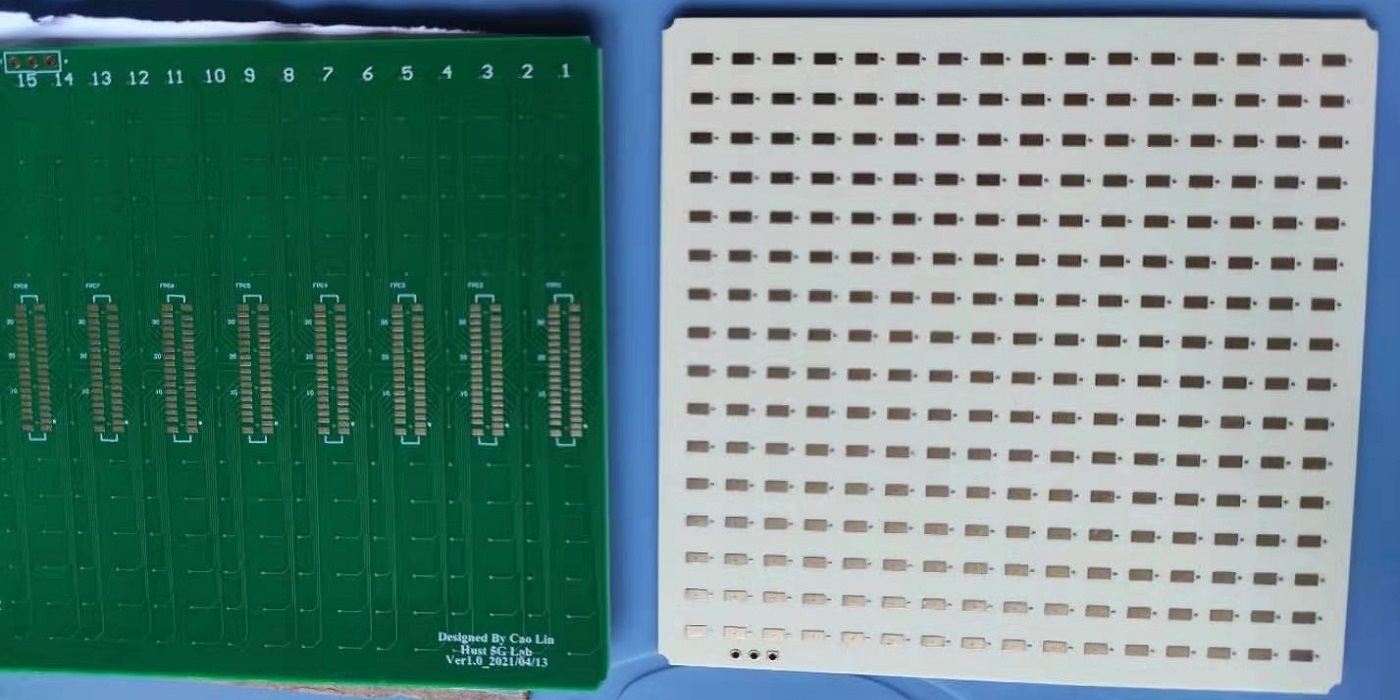
\includegraphics[width=0.3\linewidth]{Figures/28-GHz-RIS-real.jpg}}
	\hfil
	\subfloat[实物立体图]{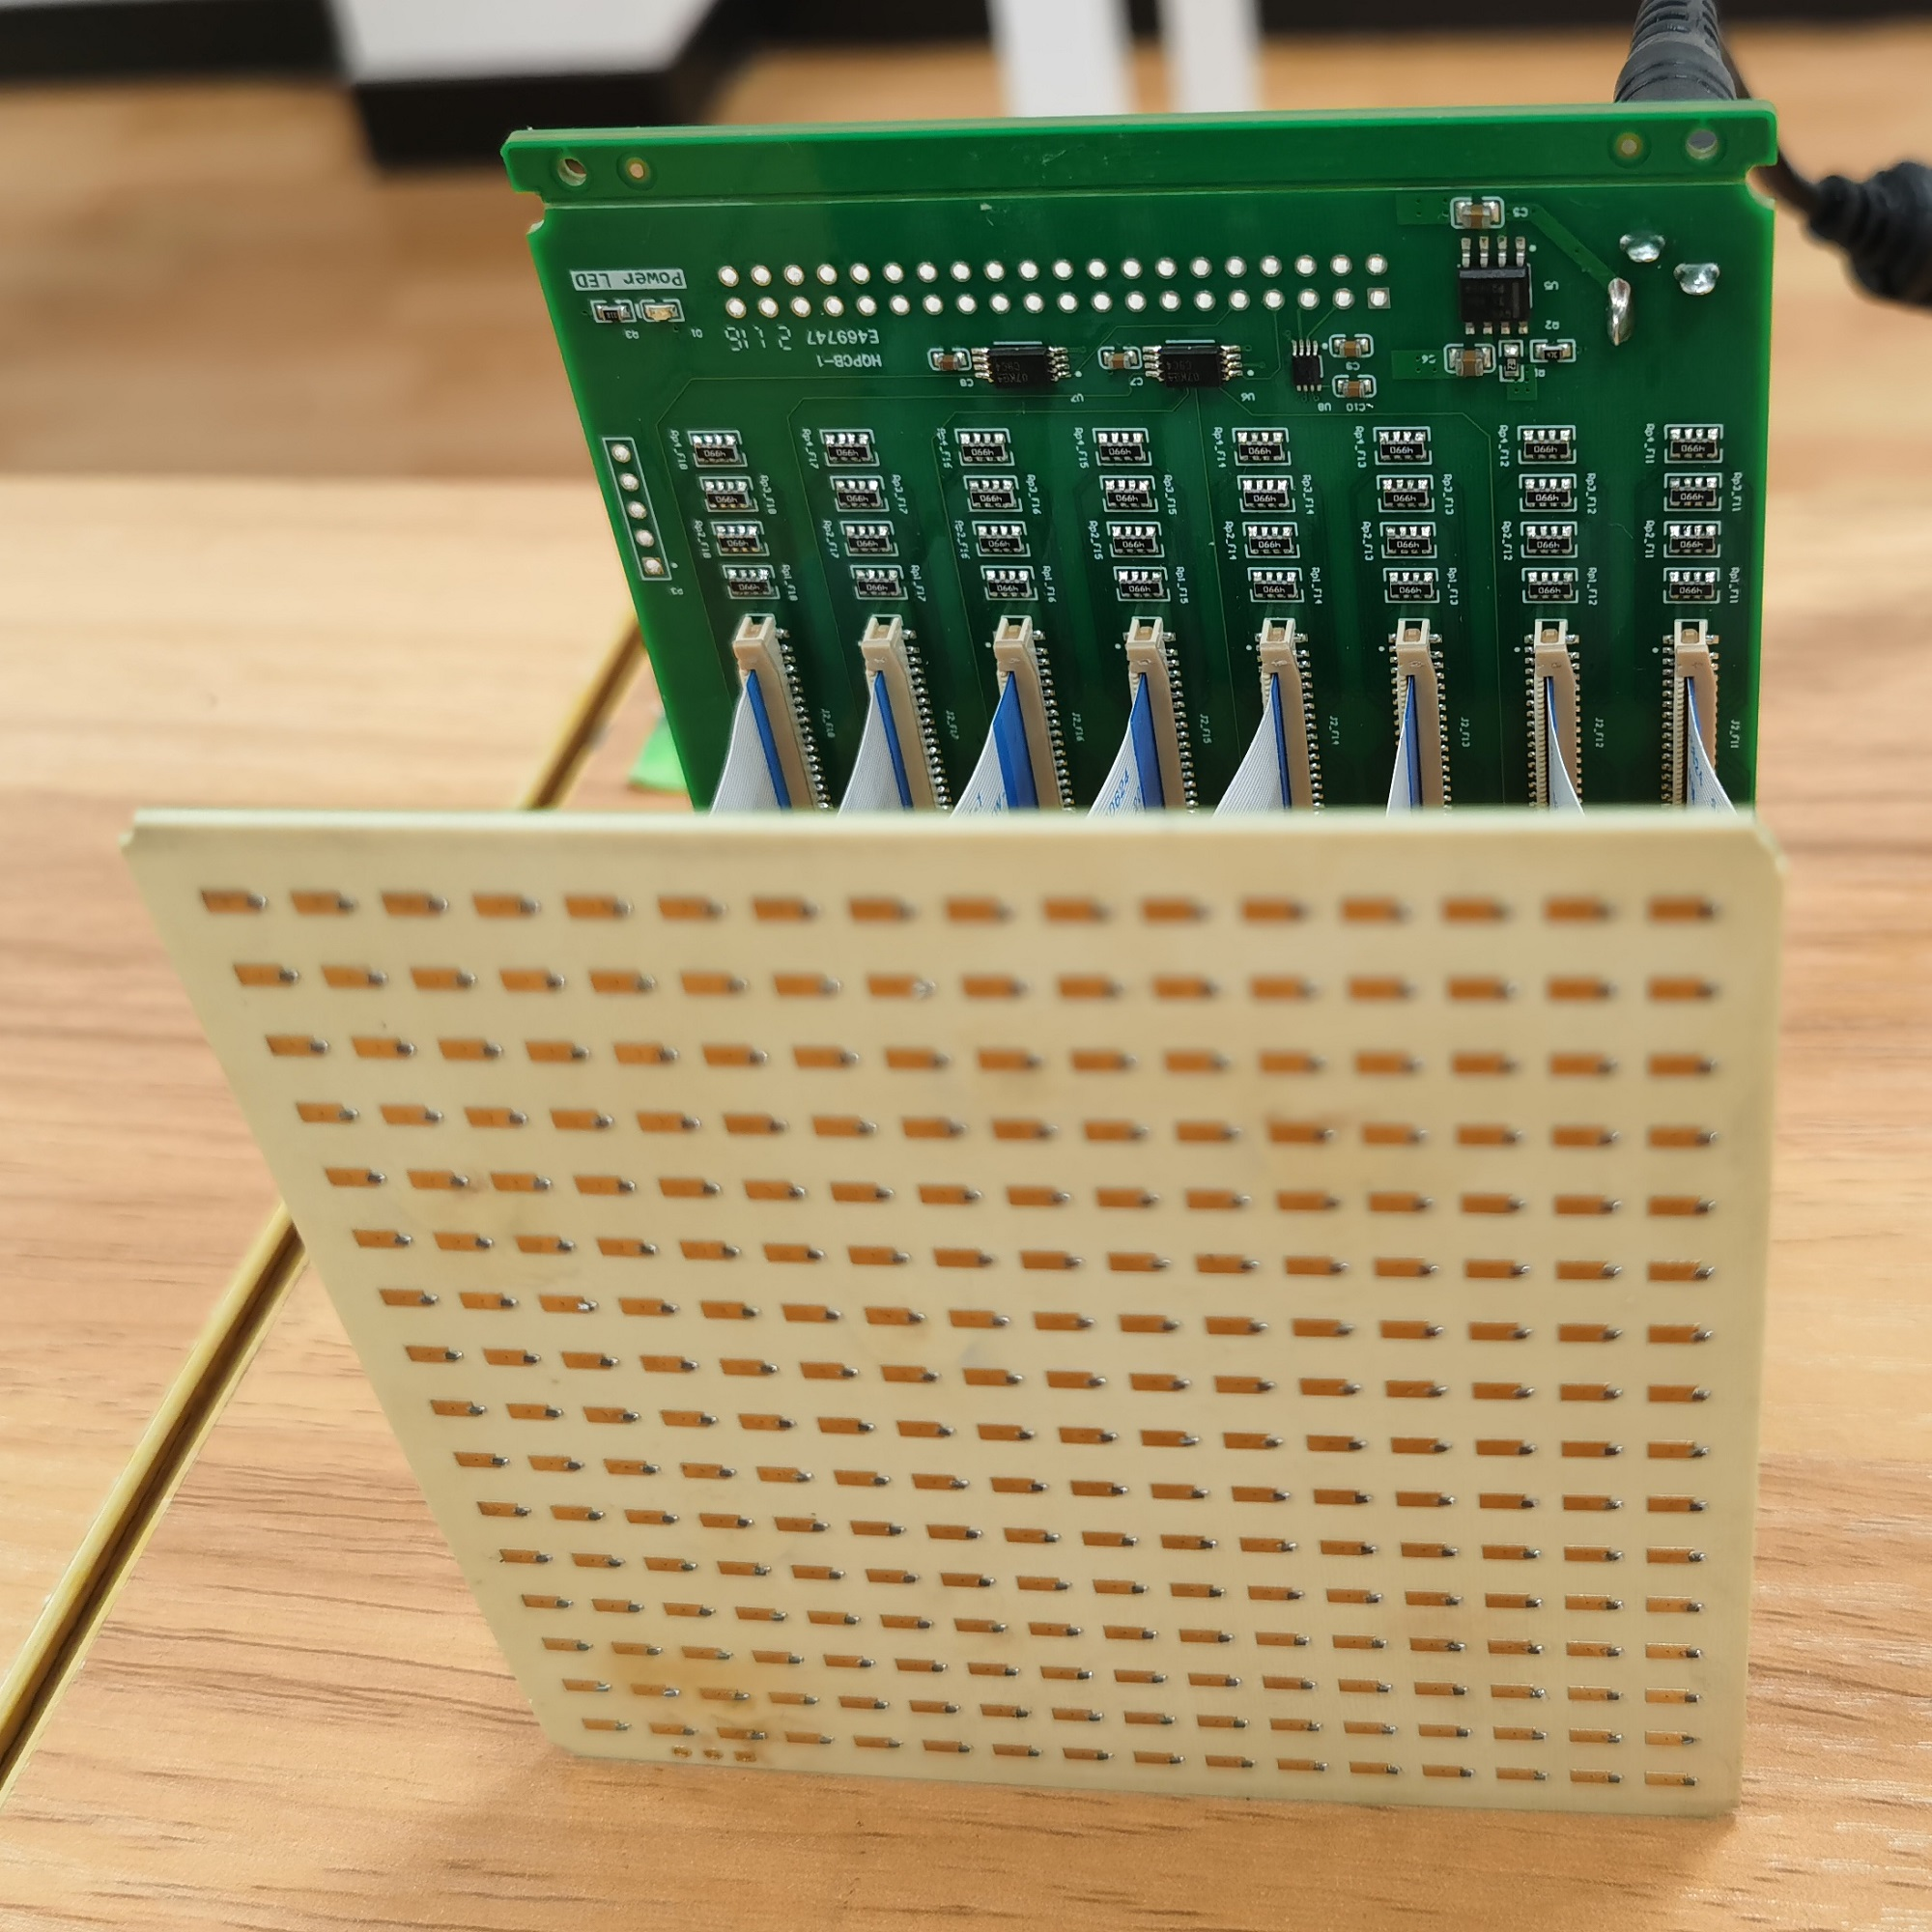
\includegraphics[width=0.3\linewidth]{Figures/28-GHz-RIS-real2.jpg}}
	\caption{28 GHz智能超表面}
	\label{fig:28-GHz-RIS}
\end{figure}

它的主要优良特性如下:
\begin{enumerate}
	\item 采用MACOM公司的PIN二极管,型号为MADP-000907-14020,工作频率可以到70 GHz。它有着极低的RC时间常数(0.1皮秒)和2至3纳秒的开关速度;
	\item 一共由$16\times16=256$个单元构成,单元数量众多,且可以独立控制,灵活性高;
	\item 28 GHz智能超表面拥有1600 MHz的工作带宽,能在主流的毫米波频段下工作;
	\item 采用模块化设计,可以多块拼接,组成大规模RIS阵列。
\end{enumerate}

\subsection{控制电路设计}

现今智能超表面的控制方法是使用一个控制器IO口控制一个反射单元,这种方法虽然简单,但是由于超表面往往有大量的电磁单元,因此需要大量的控制器IO口资源。例如,对于具有$L$个单元的智能超表面,就需要$L$个控制引脚,特别地,如果引入模拟控制,则需要$L$路数模转换电路,这会导致硬件实现成本居高不下。
为了高效的控制\autoref{subsec:28-GHz-RIS}中选择的智能超表面,本文提出了两种高效的智能超表面控制方法,并基于此设计了一款模块化的智能超表面控制电路。
下面首先介绍行列扫描控制方法。

\subsubsection{行列扫描控制方法}

生活中有许多常见的产品是由行列扫描驱动的,例如键盘、LED点阵显示屏和液晶显示器等。受此启发,本文将行列扫描的技术运用在智能超表面的控制上,提出了提供一种有源矩阵式的行列扫描控制方案,从而实现利用少数控制器引脚控制大规模的反射阵列的目的,节省了智能超表面系统的成本,提高了控制器的利用效率。

\begin{generalfig}[htb]{基于行列扫描的智能超表面控制方法示意图}{fig:MOS}
	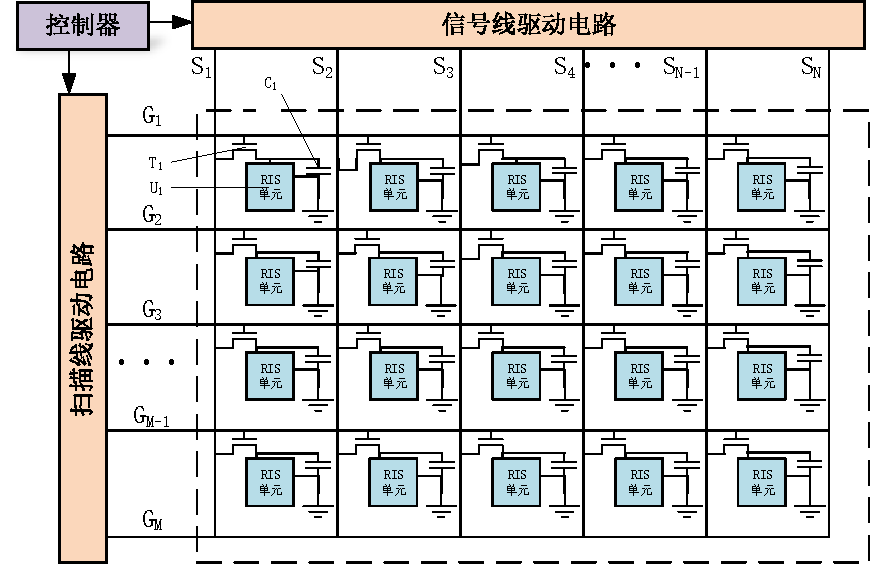
\includegraphics[width=0.8\linewidth]{Figures/MOS.pdf}
\end{generalfig}
如\autoref{fig:MOS}所示为本文设计的基于行列扫描的智能超表面控制方法示意图,图中控制器负责运行智能超表面的控制算法,将运算得到的反射系数矩阵输出给扫描线驱动电路和信号线驱动电路。
剖析左上角的第一个RIS单元及其控制电路:
$U_1$为设计的RIS单元,与它并联的是一个保持电容$C_1$。
单元$U_1$由晶体管$T_1$来控制加载的电压。
当单元$U_1$的行扫描信号脉冲结束后,保持电容$C_1$仍能保持单元$U_1$两端的电压,从而为RIS单元提供持续的驱动电压,直到下一次选通到来。

具体来说,按照本文中的设计,对$M$行$N$列的智能超表面阵列进行$Q ~ \mathrm{bit}$的控制$(Q \ge 1)$时,控制器向扫描线驱动电路发送扫描信号,由扫描线驱动电路选通某一行RIS单元(图中$G_1,G_2,G_3,\cdots,G_{M-1},G_M$)。
接着,控制器向信号线驱动电路发送此行RIS的控制信号,信号线驱动电路在$S_1,S_2,S_3,\cdots,S_{N-1},S_N$上加载$Q ~ \mathrm{bit}$的模拟信号作为控制电压。
此时,被选中行的MOS管导通,电压加载到RIS单元上。
未选通的行的MOS管关断,控制电压由RIS单元对应的保持电容保持。
需要注意的是,控制器需要对RIS面板定时刷新,使保持电容的电压维持在较为稳定的水平。

\begin{generalfig}[htb]{基于行列扫描的智能超表面单元}{fig:MOS-single}
	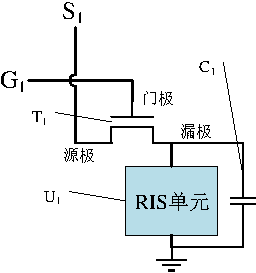
\includegraphics[width=0.4\linewidth]{Figures/MOS-single.pdf}
\end{generalfig}

\autoref{fig:MOS-single}为基于行列扫描的智能超表面的左上角单元示意图,接下来考虑保持电容容值$C_1$的设计。
仍然设RIS面板的尺寸为$M$行$N$列,对RIS面板进行刷新时,每秒更新$f$次,则每次的更新时间为$T=1/f$,即:每帧(Frame)更新时间为$T$,每行更新时间为$T_h=T/M$。
每次刷新时电容的充电时间$dt_{charge}=T_h$,而电容需要保持的时间为$dt_{hold}=T-T_h$。
设RIS单元的阻值为$R_\mathrm{RIS}$,MOS管$T_1$关断时的RIS单元的电流和MOS漏电流之和为$I_{leak}$,关断时允许的电压降为$dV_{hold}$,正常工作时RIS单元的电压为$V_{hold}$。
需要充电的电压$dV_{charge}$为信号线电压与RIS单元电压的电压差,即为晶体管的$V_{ds}$,有:
\begin{equation}
	dV_{charge} = V_{ds}
	\label{eq:V_charge}
\end{equation}
导通充电时,假设充电电流为$I_{charge}$,分析电容充电电荷,有:
\begin{equation}
	I_{charge} \cdot t_{charge}>C_1 \cdot dV_{charge}
	\label{eq:I_charge}
\end{equation}
为保证控制效果,使保持电容的电压维持在较为稳定的水平,要求:
\begin{equation}
	dV_{hold} \le 0.05 \cdot V_{hold}
	\label{eq:V_hold}
\end{equation}
即电压变化率不超过5\%。
关断保持时,对电荷变化建立不等式:
\begin{equation}
	I_{leak} \cdot t_{hold} < C_1 \cdot dV_{hold}
	\label{eq:I_leak}
\end{equation}
其中$I_{leak} = \frac{V_{hold}}{R_\mathrm{RIS}}$。
联立\autoref{eq:V_charge},\autoref{eq:I_charge},\autoref{eq:V_hold}和\autoref{eq:I_leak},可以得到$C_1$的取值范围为:
\begin{equation}
	\frac{20(M-1)}{M} \cdot \frac{T}{R_\mathrm{RIS}} < C_1 < \frac{MI_{charge}T}{V_{ds}}
	\label{eq:C1_value}
\end{equation}

然而对于驱动PIN二极管使能的超表面单元来说,\autoref{eq:C1_value}可能是无解的,这是因为包含PIN二极管的单元的导通电阻$R_\mathrm{RIS}$太小,这时候需要对\autoref{fig:MOS-single}中的电路结构进行改进。

\autoref{fig:Amp}所示为第1行第1列一个RIS单元及采样保持装置的改进结构。
其中场效应管$T_1$的栅极接扫描线$G_1$,源极接信号线$S_1$,漏极接保持电容$C_1$,并连接到运算放大器$A_1$的同向输入端,运算放大器处于单位跟随状态,输出接RIS单元,同时接反向输入端。

\begin{generalfig}[htb]{带采样保持器的智能超表面单元}{fig:Amp}
	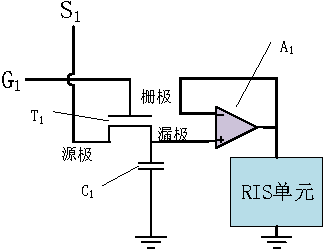
\includegraphics[width=0.5\linewidth]{Figures/Amp.pdf}
\end{generalfig}

选通时间内,场效应管处于导通状态,信号线上的电压被加载到运算放大器的同向输入端并给电容充电;电压经过运算放大器跟随后加载到RIS单元上。
关断时间内,场效应管处于关断状态,由于运算放大器的输入电阻很大,用这种方法可以保持更长时间,且不受RIS单元阻抗的影响。
这种改进电路降低刷新频率,提高稳定性,并且由于运算放大器的输出驱动能力较强,这种电路结构可以驱动阻抗小的RIS单元。

使用行列扫描控制方法可以IO口的数量得到锐减,1 bit控制时容易得出以下的结论:
\begin{enumerate}
	\item 若扫描线驱动电路一对一接入控制器,则一共需要$M+N$个IO口;
	\item 若扫描线驱动电路采用译码逻辑电路,则一共需要$\log_{2}{M}+N$个IO口;
	\item 若扫描线驱动电路采用移位寄存器电路,则一共需要$N+1$个IO口。
\end{enumerate}

\subsubsection{移位寄存器控制方法}

行列控制可以大大减少IO口数量,但白璧微瑕,这种方案需要对智能超表面定时刷新。所以,本小节提出了一种使用移位寄存器的控制方法,无需刷新就可以稳定地保持电平,在原理上更为简单。
移位寄存器是一种数字电路类型,使用多个触发器级联构成,其中一个触发器的输出连接到下一个触发器。
它们共享单个时钟信号,时钟触发会导致系统中存储的数据从一个位置转移到下一个位置。

\begin{generalfig}[htb]{4位的串入并出移位寄存器}{fig:4-Bit_SIPO_Shift_Register}
	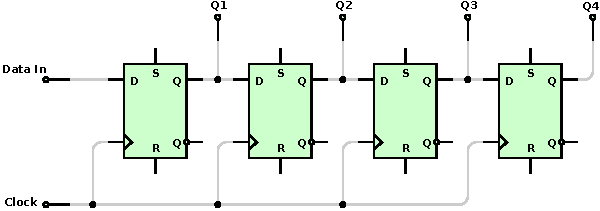
\includegraphics[width=0.8\linewidth]{Figures/4-Bit_SIPO_Shift_Register.pdf}
\end{generalfig}

\autoref{fig:4-Bit_SIPO_Shift_Register}为串入并出形式的移位寄存器接法,可以将输入的串行数据以并行格式输出。串行通信要求的几位数据完成输入之后,就可以在输出端的各位同时读出并行数据。
在这种配置中,每个触发器是边沿触发。所有触发器都以给定的时钟频率运行。每个输入位在$n$个时钟周期后将移动到第$n$个触发器的输出端,导致并行输出。

若使用$a~\mathrm{bit}$的移位寄存器,$b$个级联作为一组控制,对于一个$M$行$N$列的智能超表面,需要的控制引脚数约为$\frac{MN}{ab}$。由此可见,这也是一种差强人意的控制方法。

\subsubsection{智能超表面控制电路}

本小节详细阐述智能超表面控制电路:首先对两种方案进行比较选择,其次给出控制电路的总体设计,然后描述各个部分的设计细节,最后给出设计结果。

\subsubsubsection{方案选择}

权衡上述方法的利弊,最终选用移位寄存器控制方法制作智能超表面的控制电路,以获得更良好的系统稳定性。
在数据更新过程中,我们希望串行数据加载过程中并行输出不应改变,故需要使用锁存或缓冲输出。
如\autoref{fig:Logic-diagram}所示,在带输出锁存的移位寄存器中,串行数据首先加载到内部缓冲寄存器中,然后在接收到输出加载信号时,将缓冲寄存器的状态复制到一组输出寄存器中。

\begin{generalfig}[htb]{带输出锁存的移位寄存器逻辑图}{fig:Logic-diagram}
	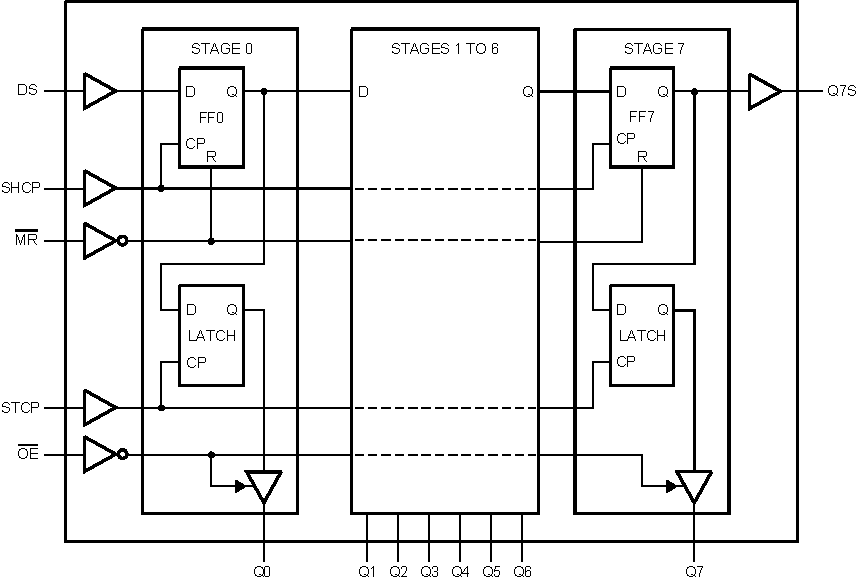
\includegraphics[width=0.8\linewidth]{Figures/Logic-diagram.pdf}
\end{generalfig}

\subsubsubsection{总体设计}

考虑到所选的智能超表面一共需要$16\times16=256$个控制信号。
综合比较控制速度和硬件复杂度,选用两片移位寄存器级联作为一组,一共16组的方案控制RIS。
为了使控制电路也能模块化组装,在设计时保持了智能超表面和控制电路的机械尺寸一致。

\begin{generalfig}[htb]{控制电路系统框图}{fig:CCB-diagram}
	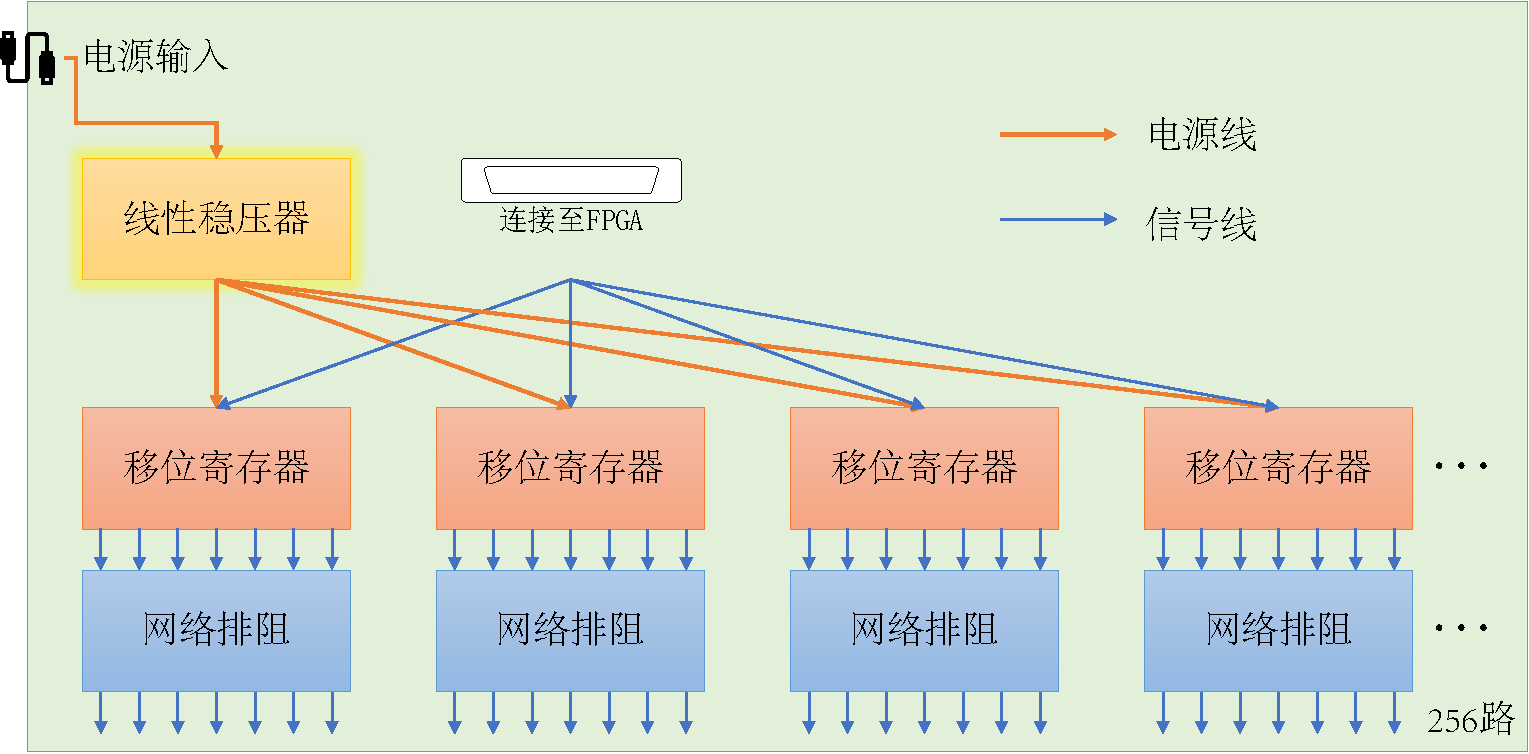
\includegraphics[width=0.8\linewidth]{Figures/CCB-diagram.pdf}
\end{generalfig}

控制电路的系统框图如\autoref{fig:CCB-diagram}所示,包括电源、移位寄存器和网络排阻几部分。
其中,电源采用低压差线性稳压器(Low-dropout regulator, LDO),以提供相较开关电源纹波更低、噪声更小的输出。
移位寄存器具有将串行信号转为并行信号的作用,图中的移位寄存器共用时钟信号,同步输出。
由于工作时PIN二极管处于导通状态,需要串联网络排阻将电流限制在4 mA左右。

\subsubsubsection{电源管理}

假设28 GHz RIS中的PIN二极管导通时的电流为$I_{work}$,供电电压为$U_{work}$,考虑极端情况,即所有单元均处于导通状态,此时RIS的总电流为:
\begin{equation}
	I_{total}=MNI_{work}
\end{equation}
总功耗为:
\begin{equation}
	P_{total}=U_{work}I_{total}=MNU_{work}I_{work}
\end{equation}
带入$M=N=16,I_{work}=4\,\mathrm{mA}, U_{work}=3.3\, \mathrm{V}$,可得:$I_{total}=1024 \, \mathrm{mA},P_{total}=3.38\,\mathrm{W}$。
由此可见,至少需要使用输出电流能力1.5 A的LDO芯片。

为保证设计的通用性,使用DC插座输入5 V直流电压,该电压作为后续LDO芯片的输入。
LDO芯片选用TPS7A7001\footnote{详细信息和数据手册请参考 https://www.ti.com.cn/product/cn/TPS7A7001 。},它是德州仪器(Texas Instruments)公司生产的一款高性能、正电压、低压降稳压器,专为 要求在高达2 A的电流下拥有超低输入电压和超低压降的应用而设计。
该器件支持低至1.425 V的单输入电压,输出电压最低可通过编程设定为0.5 V。
输出电压可使用外部电阻分压器进行设置。TPS7A7001具有超低压降,非常适用于输出电压与输入电压极为接近的应用。
此外,TPS7A7001还具有使能引脚以便在关断模式下进一步降低功率耗散。

\begin{generalfig}[htb]{TPS7A7001应用电路图}{fig:TPS7A7001}
	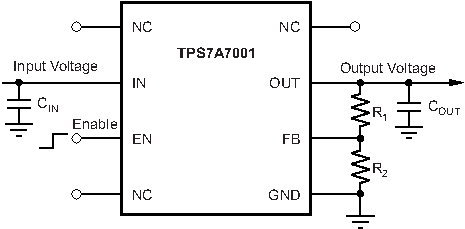
\includegraphics[width=0.6\linewidth]{Figures/TPS7A7001.pdf}
\end{generalfig}

如\autoref{fig:TPS7A7001}所示,为了使LDO稳定工作,需要选取合适的输入电容$C_\mathrm{IN}=22\,\mathrm{\mu F}$和输出电容$C_\mathrm{OUT}=100\,\mathrm{\mu F}$。
FB引脚上的电压将设置输出电压$V_\mathrm{OUT}$,并由$R_1$和$R_2$的值确定如下:
\begin{equation}
	V_\mathrm{OUT} = 0.5 \times \left(1+\frac{R_1}{R_2}\right)  
	\label{eq:TPS7A7001}
\end{equation}
反之,可以通过\autoref{eq:TPS7A7001}和需要的输出电压$V_\mathrm{OUT}$来计算$R_1$和$R_2$的值。本设计中$V_\mathrm{OUT} = 3.3 \, \mathrm{V}$,在E96系列电阻中尝试,选用$R_1=169\, \mathrm{k}\Omega , R_2=30.1\, \mathrm{k}\Omega $,满足设计要求。

\subsubsubsection{串并转换}

本设计选用了安世半导体(nexperia)生产的型号为74LVC595ABQ\footnote{详细信息和数据手册请参考 https://www.nexperia.cn/product/74LVC595ABQ 。}的移位寄存器。
它是具有存储寄存器和三态输出的8位串行至并行移位寄存器。
其中移位操作和存储寄存器都具有单独的时钟,并且该器件具有串行输入(DS)和串行输出(Q7S),以实现级联和异步重置,满足本设计的需求。

对于级联应用而言,在第一个时钟上升沿DS输入的“引脚电平值”,需要在第8个时钟上升沿时刻时,被移位至第一片74LVC595ABQ的第8位的寄存器中;
在第9个时钟上升沿时刻,该“值”需要被推移至下一片级联的74LVC595ABQ的第一位寄存器中。
这样,就需要在第9个SHCP上升沿之前,将该“值”呈现在第二片的DS引脚上,并等待第9个SHCP上升沿时刻的到来。
74LVC595ABQ逻辑门的处理方法是引入Q7S这个引脚,在第8个SHCP时刻后,将该值呈现在第二片的DS引脚上。如\autoref{fig:Timing-diagram}所示为74LVC595ABQ的时序图。
因此,若要实现74LVC595ABQ串并转换的级联扩展,只需将数据DATA信号连接至第一片74LVC595ABQ的DS引脚,并将第一片74LVC595ABQ的Q7S输出连接至第二片74LVC595ABQ的DS引脚,依次类推。
而各74LVC595ABQ的SHCP,STCP信号连接至统一的信号端。
\autoref{fig:2shift}为典型的二级74LVC595ABQ级联电路示意图,它能够将FPGA输出的串行信号转化16路并行信号,相当于实现了FPGA引脚的拓展,减小了系统对FPGA本身引脚数量的需求。

\begin{generalfig}[htb]{两片8位移位寄存器级联原理图}{fig:2shift}
	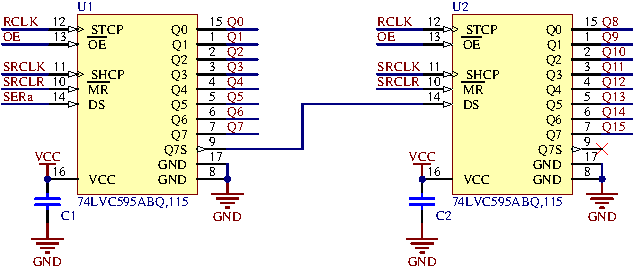
\includegraphics[width=0.8\linewidth]{Figures/2shift.pdf}
\end{generalfig}

在3.3 V供电条件下,74LVC595ABQ可以在180 MHz的时钟速率下运行。由于没有进行等长布线,为了约束时序并保持信号完整性,将时钟频率设为$f_{clk}=50 \,\mathrm{MHz}$,则刷新一次的时间$T=16/f_{clk}=0.32 \,\mathrm{\mu s}$,可以实现实时调控的目标。

\subsubsubsection{小结}

本小节详细描述了智能超表面控制电路的设计,为了增强FPGA IO引脚的驱动能力,驱动电路还采用了缓冲芯片SN74LVC2T45\footnote{详细信息和数据手册请参考 https://www.ti.com.cn/product/cn/SN74LVC2T45 。}、时钟分配芯片CDCLVC1104\footnote{详细信息和数据手册请参考 https://www.ti.com.cn/product/cn/CDCLVC1104 。},这里不再展开叙述。
控制电路的原理图详见附录~\ref{sec:schdoc},\autoref{fig:CCB_ALL}(a)为其三维仿真图,\autoref{fig:CCB_ALL}(b)为其实物图。

\begin{figure}[htb]
	\centering
	\subfloat[三维仿真图]{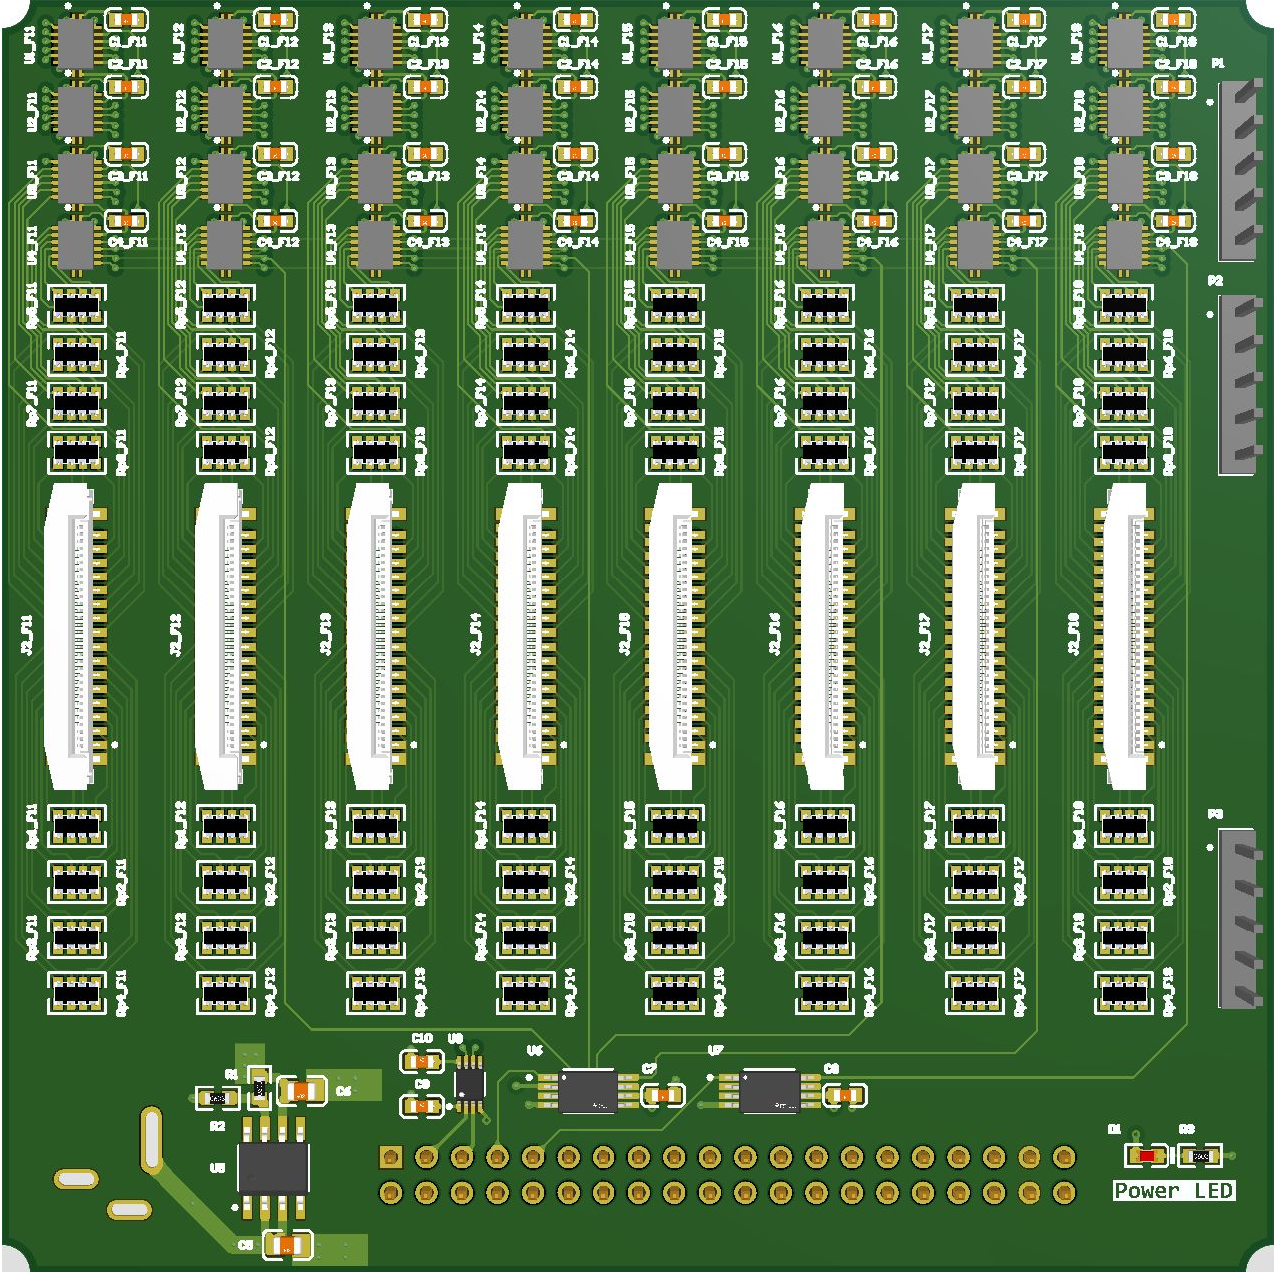
\includegraphics[width=0.4\linewidth]{Figures/CCB_3D.pdf}}
	\hfil
	\subfloat[实物图]{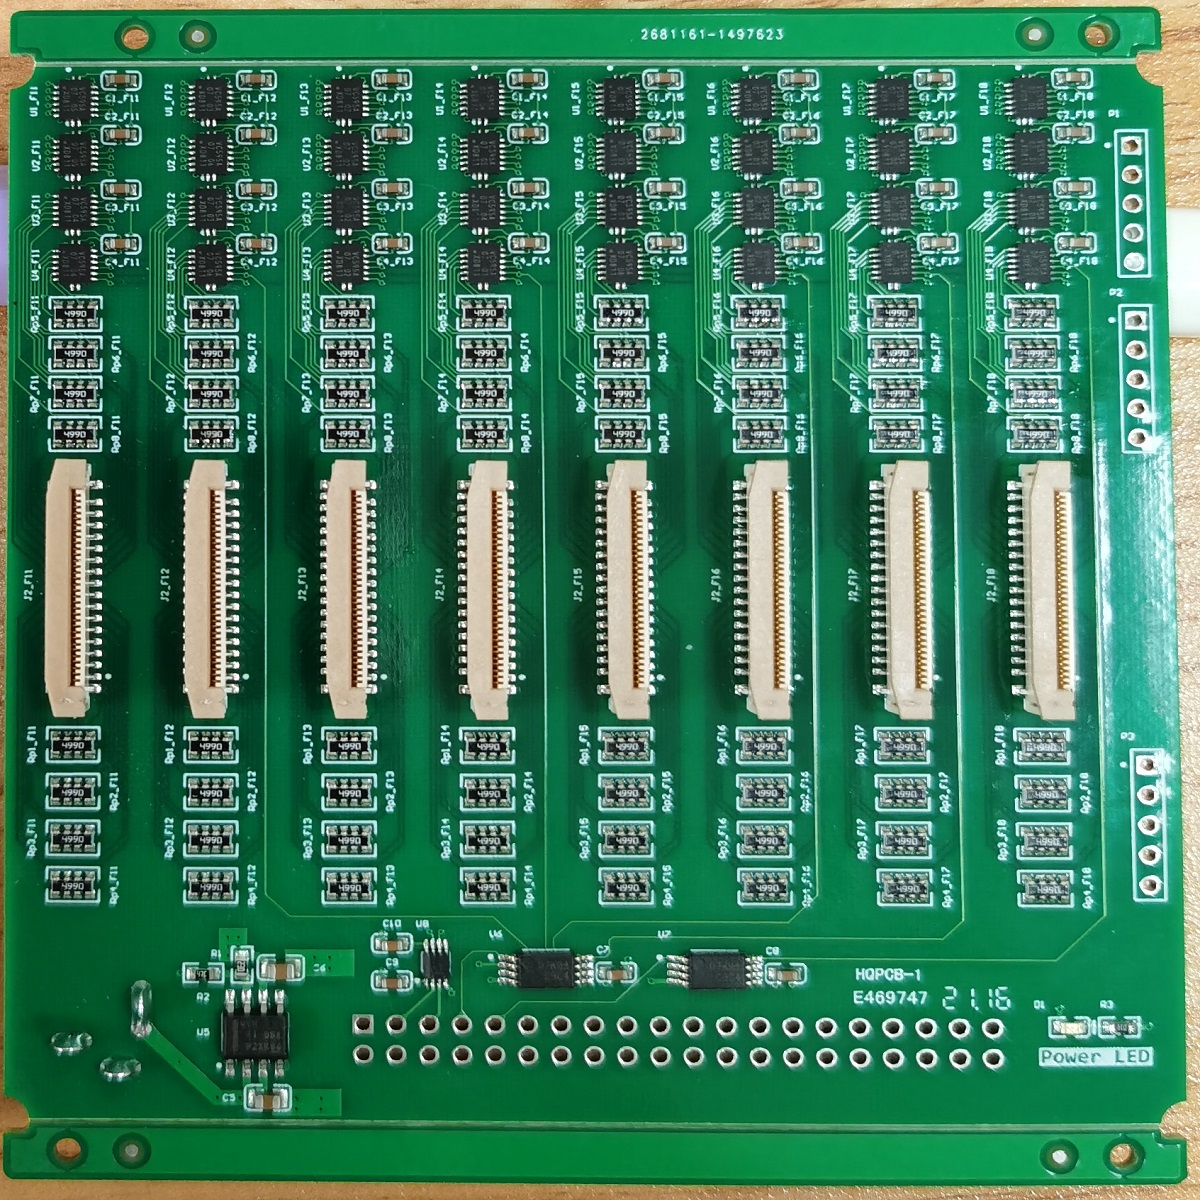
\includegraphics[width=0.4\linewidth]{Figures/CCB_real.jpg}}
	\caption{智能超表面控制电路}
	\label{fig:CCB_ALL}
\end{figure}

\subsection{驱动、固件设计}

本小节将详述智能超表面驱动、固件的设计。驱动程序和固件是一个复杂系统的“地基”,没有它就不能建成高楼大厦。本节中,我将从设计思路入手,把驱动的设计过程和实现方法娓娓道来。

\subsubsection{设计思路}

首先需要控制移位寄存器。根据\autoref{fig:Timing-diagram}即74LVC595ABQ的时序图,在顶级模块声明移位时钟,数据和锁存引脚,以及系统时钟,然后使用状态机,定义空闲状态为锁存状态,即不存在新的数据输入,这时移位寄存器模块不工作。定义更新状态,此时新的数据输入模块,模块将输入的并行数据按照\autoref{fig:Timing-diagram}串行输出,最后更新锁存引脚。

\begin{generalfig}[htb]{74LVC595ABQ时序图}{fig:Timing-diagram}
	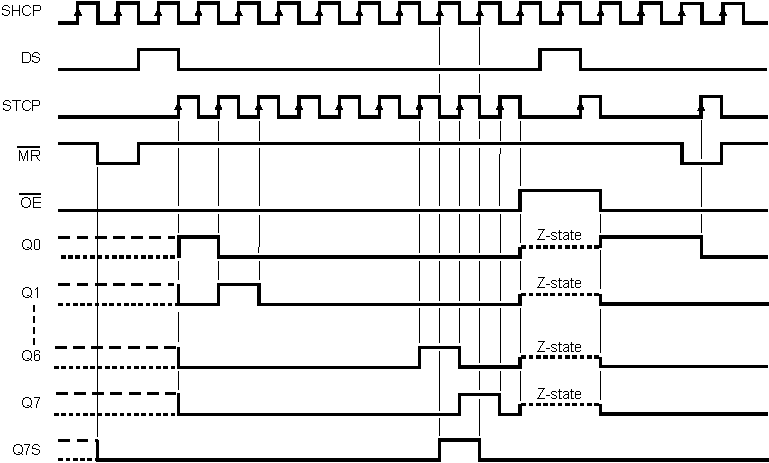
\includegraphics[width=0.8\linewidth]{Figures/Timing-diagram.pdf}
\end{generalfig}

其次要控制的是移位寄存器模块和顶层之间的通信,这里使用的是赛灵思公司提供的AXI总线。
AXI(Advanced eXtensible Interface)本是由ARM公司提出的一种总线协议, Xilinx从 6 系列的 FPGA 开始对 AXI 总线提供支持,目前使用 AXI4 版本。
数据可以同时在主设备和从站之间的双向移动,数据传输大小可以变化。
在顶层的基于C语言或Free RTOS操作系统的控制软件中,只需要向移位寄存器模块IP的相应地址写入控制数据即可实现对智能超表面的控制。

考虑到底层的控制逻辑需要并行输出,顶层又需要做算法的执行和无线通信,所以选择了赛灵思公司的Zynq$^\circledR$-7000 SoC\footnote{详细介绍可参考 https://china.xilinx.com/products/silicon-devices/soc/zynq-7000.html 。}作为主控制器。
本系列处理器集成了ARM$^\circledR$处理器的软件可编程性与Xilinx FPGA的硬件可编程性,不仅可实现重要分析与硬件加速,同时还在单个器件上高度集成 CPU、DSP、ASSP以及混合信号功能。
其框图如\autoref{fig:zynq-7000}所示,该FPGA PS部分具有两个ARM Cortex-A9高性能应用级ARM处理器,PL部分有171.9 k个LUT,343.8 k个触发器。
所选用的核心板有1 GB DDR3 SDRAM,4 GB eMMC,资源丰富。
它还具有高速接口与可编程逻辑进行通信,满足设计需求。

\begin{generalfig}[htb]{Zynq-7000 SoC框图}{fig:zynq-7000}
	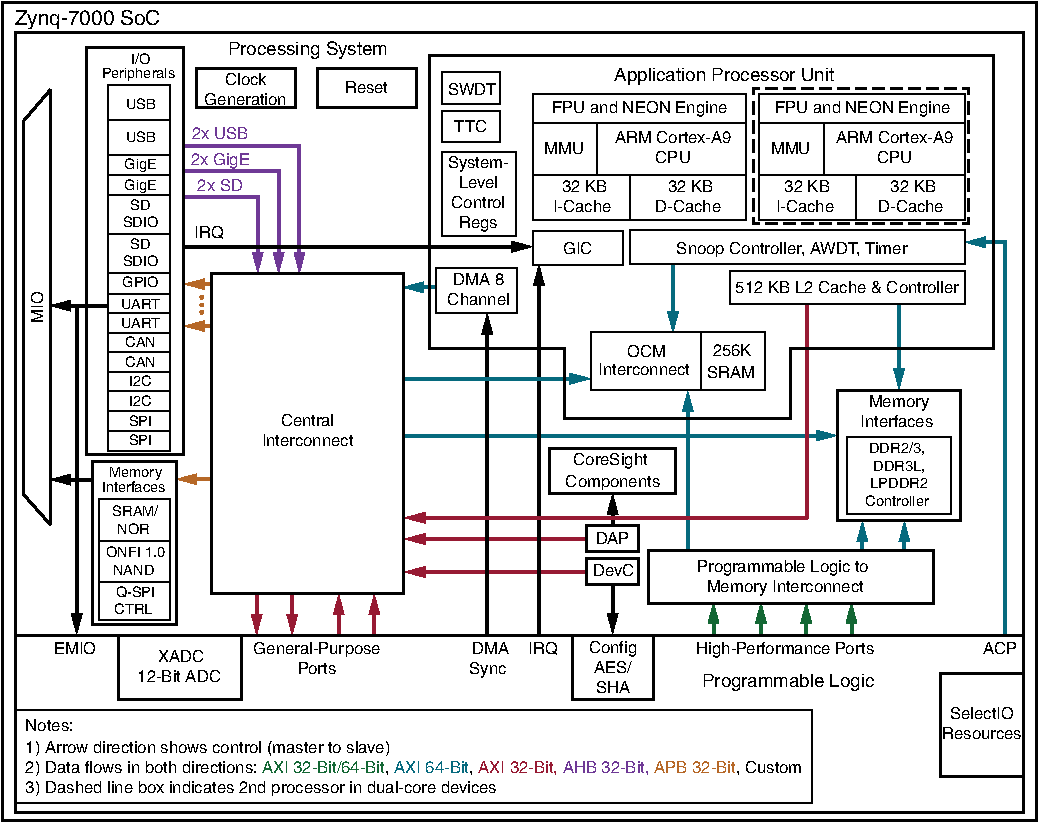
\includegraphics[width=0.8\linewidth]{Figures/zynq-7000.pdf}
\end{generalfig}

\subsubsection{设计流程}

进入赛灵思Vivado开发平台后,首先点击新建工程,确定工程的名字和路径之后,下一步是器件选型。
本设计选用的FPGA型号为Zynq-7035,因此芯片型号为xc7z035ffg676-2。
配置好器件型号之后,即完成了工程的创建,如\autoref{fig:FinishCreate}所示。

\begin{generalfig}[htb]{完成工程创建}{fig:FinishCreate}
	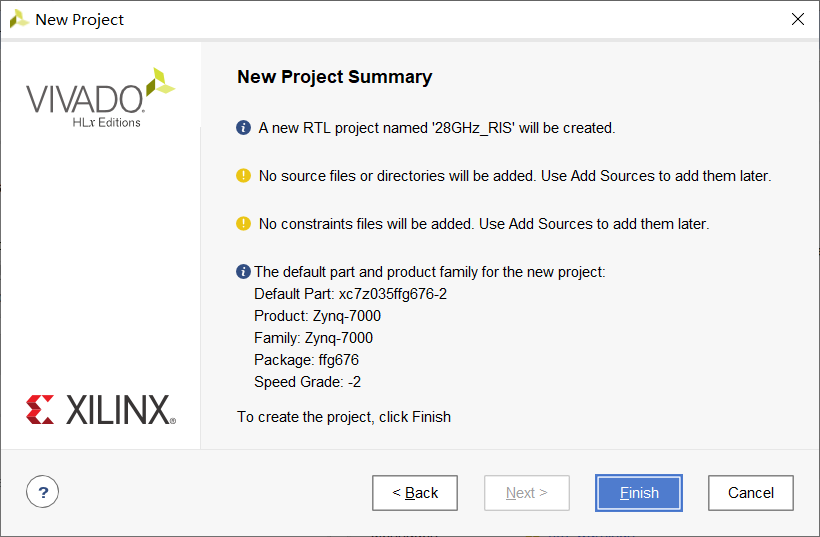
\includegraphics[width=0.8\linewidth]{Figures/FinishCreate.png}
\end{generalfig}

进入新的Vivado工程之后,我们选择添加Block Design,因为本系统是软硬件协同的,需要用到处理器,因此选用Block Design模块化设计。
添加好之后即添加IP、配置IP并连线、输出等等。
选择让Vivado自动生成顶层Verilog代码,即可完成硬件部分的逻辑设计,顶层Wrapper将会自动生成。
完成后的设计图如\autoref{fig:Block_diagram}所示。

\begin{generalfig}[htb]{FPGA固件Block Diagram}{fig:Block_diagram}
	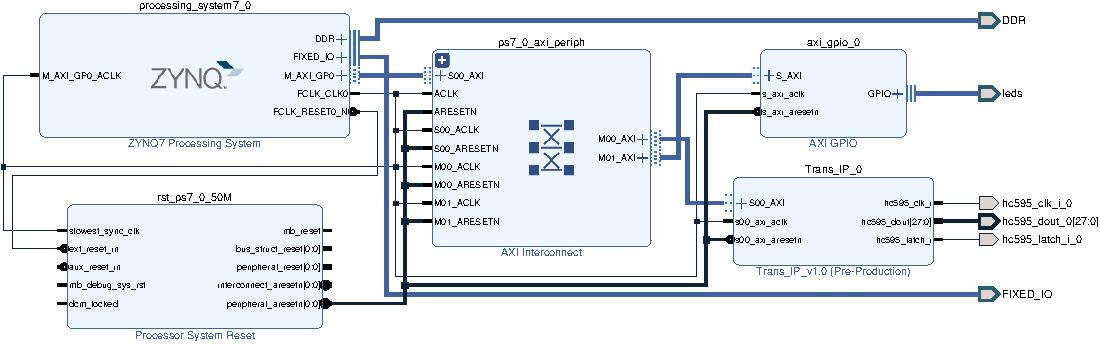
\includegraphics[width=\linewidth]{Figures/Block_diagram.pdf}
\end{generalfig}

在设计每一个模块时,需要对模块进行功能仿真,Xilinx的Vivado平台自带仿真系统,也可以使用业界常用的Modelsim进行仿真。本设计使用Modelsim进行综合前仿真,以验证功能正确性。
经过修改验证,得到如\autoref{fig:Modelsim}所示的正确的仿真波形。
蓝色标记之间展示的是一个完整的8位移位操作。
此仿真使用的是50 ns时钟周期,符合实际FPGA使用的20 MHz时钟。
仿真显示,需要大约89个时钟来处理一次输出操作,即约为4.45 us。

\begin{generalfig}[htb]{移位寄存器功能仿真}{fig:Modelsim}
	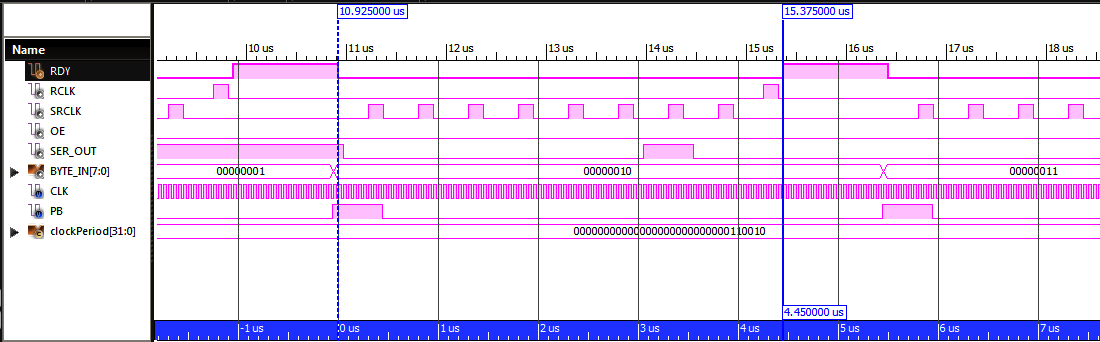
\includegraphics[width=\linewidth]{Figures/Modelsim.png}
\end{generalfig}	

\autoref{fig:Modelsim}中的信号描述如下:
\begin{itemize}
	\item {\itshape RDY}:高电平表示移位寄存器模块是空闲的,准备好处理输出要求,低电平表示正在输出。
	\item {\itshape RCLK}:发送到移位寄存器的信号,上升沿时输出寄存器从内部缓冲寄存器读取数据并输出。
	\item {\itshape SRCLK}:发送到移位寄存器的信号,上升沿时指示移位寄存器从串行输入读取,将其推入LSB,进行移位操作。
	\item {\itshape OE}:发送到移位寄存器的信号,该信号将移位寄存器输出设置为高阻态(禁用)或输出启用。这是一个低有效的信号。
	\item {\itshape SER\_OUT}:发送到移位寄存器的串行信号。
	\item {\itshape BYTE\_IN}:一个8位值,它被送入FPGA的移位寄存器模块中。
	\item {\itshape CLK}:FPGA逻辑的时钟。
	\item {\itshape PB}:为仿真创建的信号,以指示模块从{\itshape BYTE\_IN}读取8位值。每次按下此按钮(信号上升沿)FPGA移位寄存器模块都被激活并指示读取{\itshape BYTE\_IN}。此外,testbench模块将{\itshape BYTE\_IN}值递增一个。
\end{itemize}

功能验证完成后,下一步进行的是引脚约束。
使用直接编写约束文件的方式,能大大提高开发效率,因为可以通过模板来快速编写约束文件。
接着需要做时序约束。使用Vivado进行开发时,一般的时序约束方法有三种。

{\bfseries 方法1:自动创建基时钟和 PLL 输出时钟}

这一方法能够自动地约束PLL的输入和输出时钟。在ALTPLL mega function 中指定的所有 PLL 参数都用于约束 PLL 的输入和输出时钟。自动更新了 ALTPLL mega function的修改。当创建 PLL 的输入和输出时钟时,不必跟踪 PLL 参数的更改或指定正确的值。为了自动约束所有输入和输出,要将 derive\_pll\_clocks 命令和 -create\_base\_clocks选项一起使用。

{\bfseries 方法2:手动创建基时钟和自动创建 PLL 输出时钟}

通过这种方法,可以手动约束 PLL 的输入时钟并且使 TimeQuest analyzer 能够自动约束 PLL 的输出时钟。除此之外,与ALTPLL mega function 中指定的输入时钟频率相反,可以指定一个不同的输入时钟频率。通过使用 ALTPLL mega function 中指定的参数自动创建 PLL 输出时钟。

{\bfseries 方法3:手动创建基时钟和 PLL 输出时钟}

通过这种方法,可以手动约束 PLL 的输入时钟和输出时钟。指定了所有的 PLL 参数并且参数值可以不同于 ALTPLL mega function 中指定的参数值。除此之外,可以尝试各种 PLL 输入和输出频率以及参数。也可以将该方法与 create\_clock 和 create\_generate\_clock 命令的组合一起使用。
由于软硬件协同设计中,PL部分的时钟由PS内的锁相环提供,因此无需在约束文件中对PL时钟做过多约束。

上述步骤配置完成后,便可以进行综合,如果需要在线调试,还需要在综合结束之后进行配置以形成ILA。\autoref{fig:RTLFigure}是设计综合后的RTL电路图。

\begin{generalfig}[htb]{智能反射面固件RTL电路图}{fig:RTLFigure}
	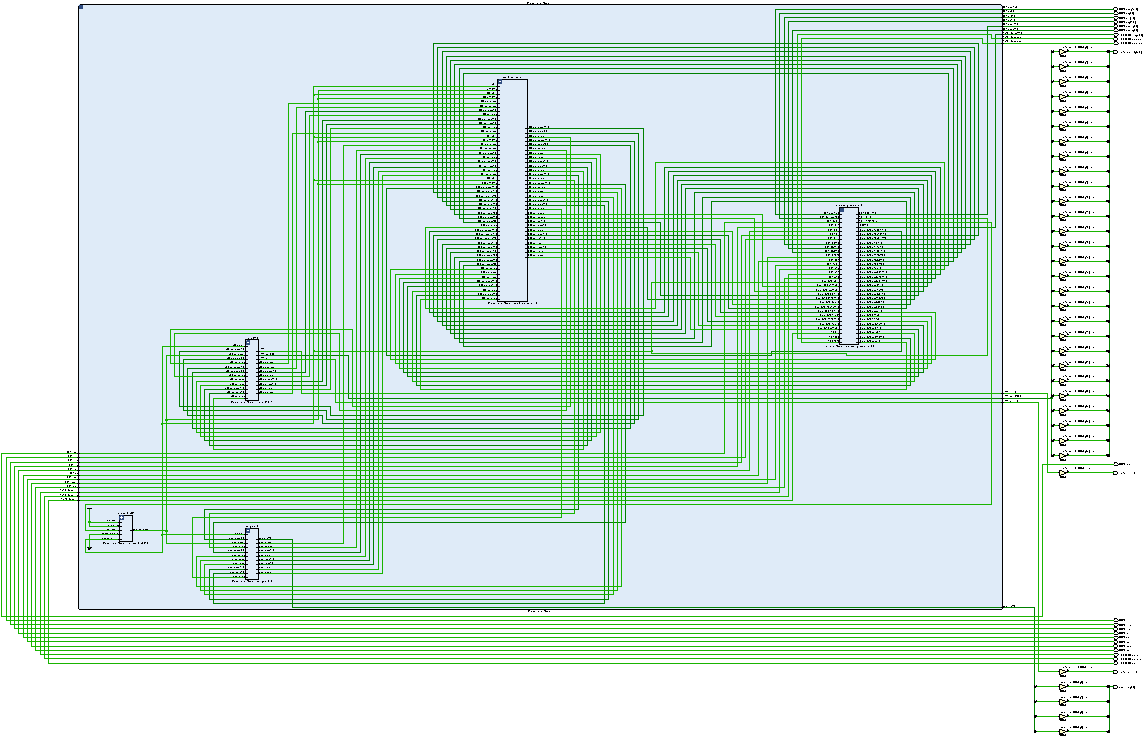
\includegraphics[width=\linewidth]{Figures/RTLFigure.pdf}
\end{generalfig}

\subsection{本章小结}

本章主要介绍了智能超表面使能的无线通信系统的实现。从超表面的选择入手,依次介绍了控制电路的设计和驱动、固件的设计。
本章还详细介绍了系统的开发流程,生成了智能超表面系统的控制固件。
这一步完成之后,便可以搭建RIS系统了。下一章将搭建智能超表面使能的无线通信系统并进行调试。

\section{系统调试}\label{sec:test}

\subsection{系统搭建}

RIS辅助无线通信系统由个人计算机(PC)、通用软件无线电外围设备(USRP)、RIS、基于FPGA的主控板和实时RIS-UE反馈模块组成。
PC、USRP和天线是发射机的主要部件,接收器由相同的部件组成。\autoref{tab:hardware}总结了系统中使用的硬件模块的细节。

\begin{generaltab}{智能超表面系统硬件模块详细信息}{tab:hardware}
	\begin{tabular}{cc}
		\toprule
		名称             & 描述                           \\ \midrule
		中央处理器       & 英特尔酷睿i7-9700处理器的电脑    \\
		软件无线电       & NI USRP-2954R                  \\ 
		上变频模块       & Sub-6 GHz 至mmWare变频器        \\
		相控阵模块       & 16通道28 GHz毫米波有源相控阵天线 \\
		FPGA模块        & 赛灵思Zynq-7035开发板            \\
		实时反馈模块     & nanoUART-wl无线串口             \\
		喇叭天线        & 27.8 GHz时的增益为21.52 dB       \\ 
		\bottomrule
	\end{tabular}
\end{generaltab}

\begin{generalfig}[htb]{智能超表面系统整体照片}{fig:TestFigure}
	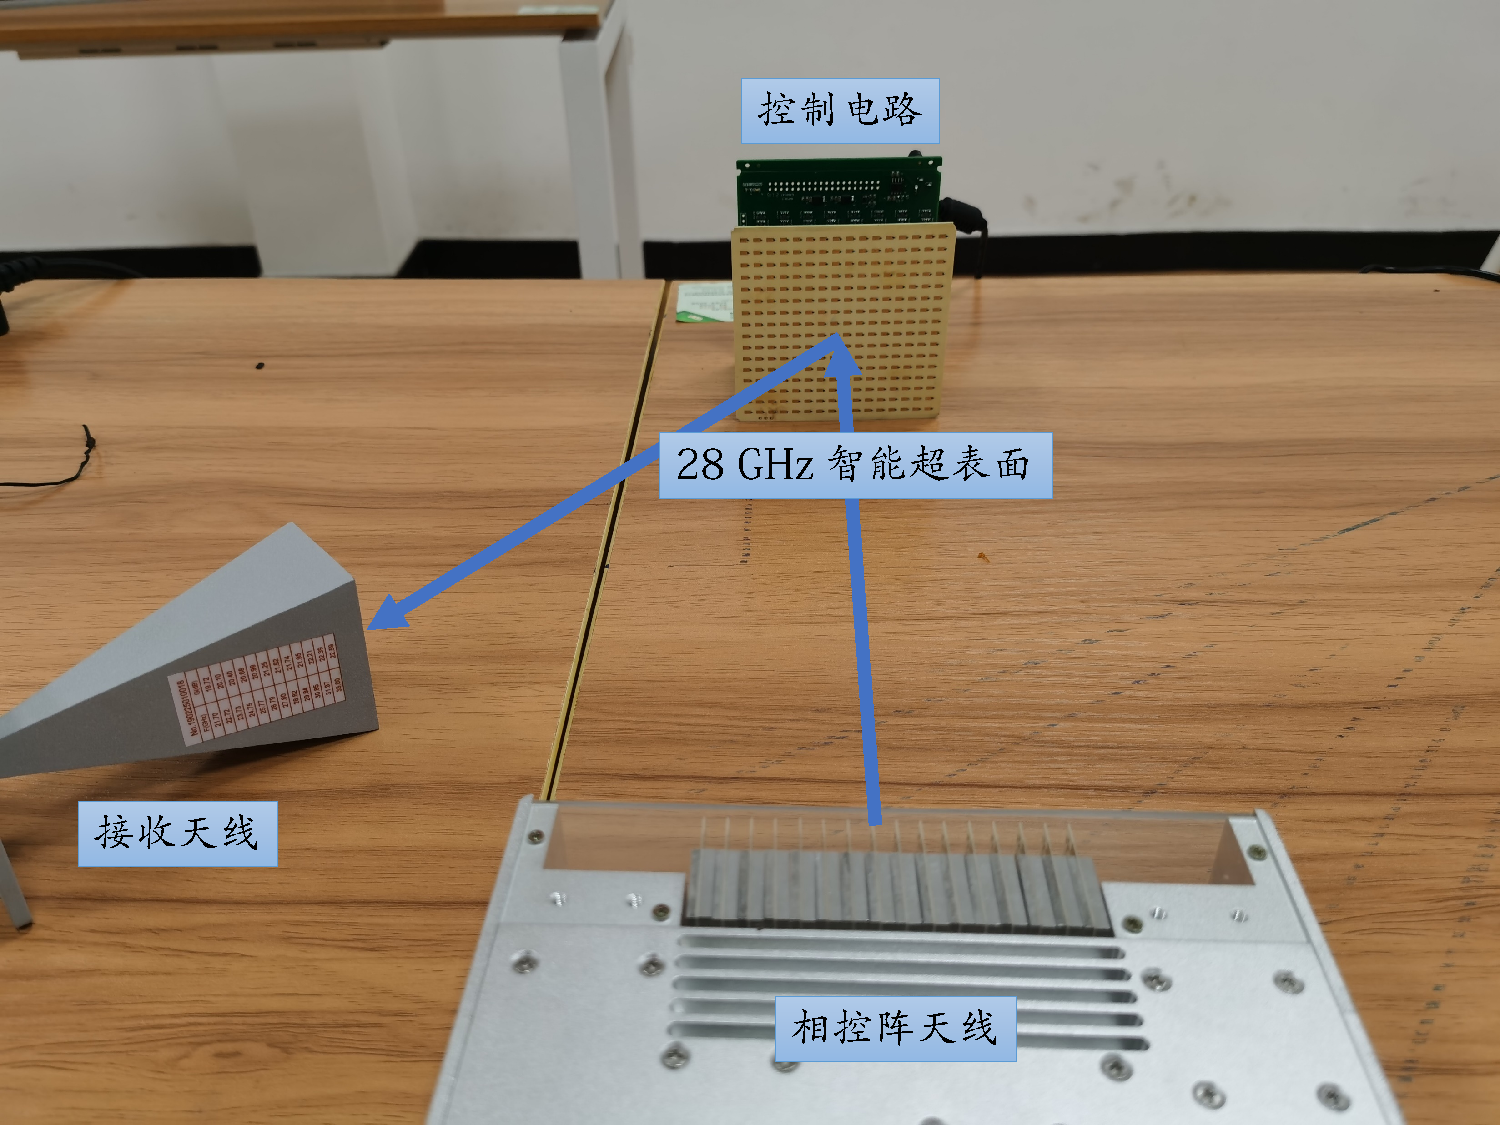
\includegraphics[width=0.8\linewidth]{Figures/TestFigure.pdf}
\end{generalfig}

发射机和接收机分别模拟基站和用户设备。
发射机使用相控阵天线发送视频流,使波束方向对准智能超表面。
数据通过用户数据报协议(UDP)传输。
智能反射面通过对表面单元反射系数的调整,将波束指向接收天线。
接收端软件无线电解码数据流并在主机上播放视频。
在原型系统中,RIS的目标是充当智能反射器,将撞击的无线信号作为波束“反射”到接收器。
为了支持反射系数的实时调整(例如,使RIS适应时变信道条件或在服务不同UE之间切换或接收终端处于移动状态),我们引入了一个反馈链路,它用无线串行端口(Wireless UART)连接RIS板和接收器。
接收机将当前信道的质量(即接收到的信号功率)反馈给FPGA主控板。
反馈可用于测量应用反射系数的有效性。如\autoref{fig:TestFigure}所示即为系统核心部分照片。

\subsection{FPGA调试与分析}

Verilog HDL是一种硬件描述语言,其最终的目的是生成硬件电路,所以与C语言不同,编程时特别在意硬件资源的消耗、时序分析以及功耗分析,如果实现相同的功能,而硬件消耗过多的话,那么这个设计就基本上是失败的。同理,时序、功耗等参数也是分析设计的重点。

在一个时序电路中,一定要满足信号的建立时间和保持时间,否则信号时序出错,数据不能正确的传达。
根据在数字电路基础这门课上学到的知识,可以得到以下的参数关系。
{\bfseries 建立时间}($T_s$:set up time)是指在时钟沿到来之前数据从不稳定到稳定所需的时间,如果建立时间不满足要求,那么数据将不能在这个时钟上升沿被稳定地送入触发器;{\bfseries 保持时间}($T_h$:hold time)是指数据稳定后保持的时间,如果保持时间不满足要求那么数据同样也不能被稳定地送入触发器。
\autoref{fig:TimingReport}为时序分析报告,可以看到,在50 MHz的时钟下,建立时间、保持时间以及时钟脉宽都满足时序约束要求。

\begin{generalfig}[htb]{FPGA片上系统时序分析报告}{fig:TimingReport}
	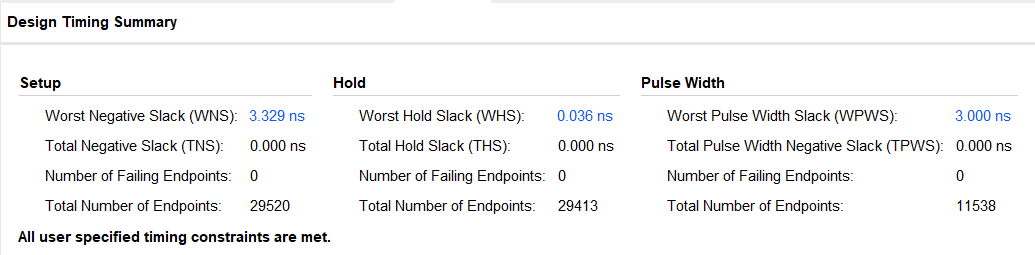
\includegraphics[width=\linewidth]{Figures/TimingReport.png}
\end{generalfig}

完成时序分析之后,需要对设计做功耗分析。
低功耗是集成电路发展的一个趋势,如果同样实现一个完好的功能,一个好的设计的功耗会非常低,那么这样的产品无疑是极有竞争力的。
因此需要研究系统功耗,在Xilinx的集成开发工具Vivado中,带有功耗分析的功能。
\autoref{fig:PowerAnalysis}所示为系统的功耗分析报告。

\begin{generalfig}[htb]{FPGA片上系统功耗分析报告}{fig:PowerAnalysis}
	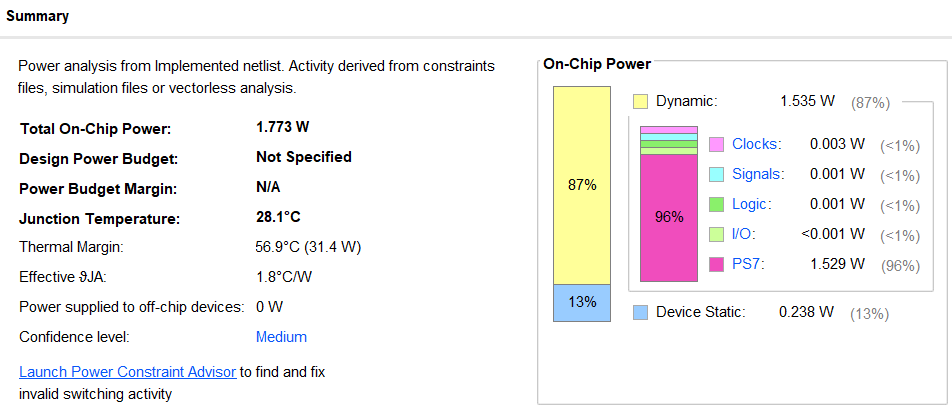
\includegraphics[width=\linewidth]{Figures/PowerAnalysis.png}
\end{generalfig}

从图中可以看出,本设计的功耗主要用在ARM核上(即PS部分),为1.529 W,达到了总功耗的96\%。
本设计没有使用很多数据传输的IP核,所以逻辑部分没有占用太多的功耗,仅为0.001 W,可以说本系统在功耗上控制得不错。

除了功耗,我们还需要关注设计所消耗的资源。
从综合到实现,Vivado工具会帮我们做一些布局布线的优化,所以综合阶段的资源占用和实现阶段的资源占用是不一样的,因此选用实现阶段后的资源报告来作为最终的资源分析。
最终消耗的FPGA硬件资源如\autoref{tab:ResourceAnalysis}所示。从图中可以看出,最终所消耗的硬件资源非常少,这是因为逻辑部分较为简单。
唯一使用较多的资源是IO口,尽管使用了高效的控制电路,IO资源仍然是最为紧张的。

\begin{generaltab}{FPGA片上系统资源使用情况表}{tab:ResourceAnalysis}
	\begin{tabular}{cccc}
		\toprule
		资源     & 已使用       & 可用      & 已使用(\%)    \\ \midrule
		LUT      & 1149        & 277400    & 0.41           \\
		LUTRAM   & 62          & 108200    & 0.06           \\
		FF       & 1607        & 554800    & 0.29           \\
		IO       & 34          & 362       & 9.39           \\
		BUFG     & 1           & 32        & 3.13           \\
		\bottomrule
	\end{tabular}
\end{generaltab}

完成实现操作后,进行比特流(Bitstream)的生成。完成所有操作后,将生成的比特流固化在FPGA核心板上的SPI Flash上,按下复位按键,系统能够实现波束扫描和波束跟踪,基础功能均得以实现。

\subsection{本章小结}

这一章简单地叙述了系统调试方面的内容。
描述了系统组成、系统搭建的过程,重点介绍了FPGA的调试与分析。最后的测试结果表明系统能实现波束调控,达到了设计目的。

\section{总结与展望}\label{sec:conclusion}

毕业设计主要内容到这里就告一段落了,下面总结一下这几个月来的学习研究工作,对未来阶段的研究工作提出一些自己的思考。

\subsection{个人总结}

这次毕业设计从2020年年底确定选题开始,到2021年5月已经半年有余,总体来说时间还是比较充裕的。
在此期间,设计工作基本能按部就班地推进,阅读论文,指定研究思路,着手系统设计,到论文撰写,查重与修改,都能在相应的时间节点之前完成。

这次毕业设计特殊的地方在于不仅仅是仿真和软件。还包含一些对硬件的调试和对系统的调试,所以整体的复杂度是挺高的。
系统的接收机发射机都是“金贵”的毫米波射频器件,价格昂贵,使用起来得颇为小心。
两端的信号处理使用的是NI公司的软件无线电,加上主机,整个系统可以说是“阵容庞大”,平日里搬运测试时,需要装满两个较大的收纳箱。
我和实验室的同窗做测试实验时,也是“累并快乐着”,特别是室外测试时,风风雨雨都是平常事。庚子年岁末,我们在国家光电研究中心和启明学院对第一版的系统做了远距离的传输测试,展鹏学长在寒风中调试设备,为了能尽快地获得实验数据,无暇顾食。
五月初,时近立夏,江城天气诡异多变,一日可见四季,我们赶在风雨稍歇的时候在实验室楼顶完成了对接收信号功率模型的测试。
看到测试的数据能验证自己的想法,心里还是很宽慰的。

在毕业设计过程中,也有过几段小插曲。
这学期刚来学校不久,我便设计好了控制电路,联系到的PCB制造厂家需要近一个月的时间才能完成采购、生产和贴片的任务,耽误了些许时间。
另外,所涉及的智能抄表面天线面板也是比较精密的电路,还需要用到特殊的高频材料,交期也很长。所幸在五月初能拿到组成系统所有模块,可以较为顺利地开始调试的工作。
这个学期,我们团队还以这个系统为原型,报名参加了“挑战杯”的比赛,相关材料的种种打磨也是费时费力的一项工作。
经过校赛、省赛的历练,我们都成长了许多,这段时间也在做最后的冲刺,愿秋天能结出胜利的果实。

忙里偷闲写下这点文字,也算是留个纪念吧。

\subsection{工作总结}

本文的主要研究内容是如何利用可编程电磁超表面增强5G信号覆盖。
文中首先介绍了电磁超表面的相关基础理论,包括广义反射定律和折射定律以及智能超表面对电磁波的调控机理的理论。
接着对RIS通信系统建模分析,解释了无源金属表面如何散射入射波,然后推导出智能超表面必须如何设计来模拟这种表面,同时控制散射波的方向性,总结了一个严格的路径损耗模型。并建立智能超表面系统的传输模型,解释了在何种条件下,系统达到最大传输速率。
随后,基于上述的理论分析,设计了一个由可编程超表面及其控制电路构成的智能反射面系统。
从超表面的选择入手,依次介绍了控制电路的设计和驱动、固件的设计。
还详细介绍了系统的开发流程,生成了智能超表面系统的控制固件。
最后简单地叙述了系统调试方面的内容。
描述了系统组成、系统搭建的过程,重点介绍了FPGA的调试与分析。

\subsection{未来工作展望}

目前,学术界和工业界对于智能超表面的研究工作正在如火如荼地进行着,相关的研究报道可谓是日新月异。
智能超表面在毫米波通信中的应用更加值得我们去探索,本文的主要内容也是围绕毫米波系统展开的。
时下,我们第二版的毫米波系统刚刚建立,通信链路刚刚调通。
接下来一段时间首要的是将控制算法部署在智能超表面控制系统上,并进行端到端的测试实验。
未来,我们会对毫米波RIS通信系统做一系列的性能测试,研究并完善现有的理论模型。

\begin{thankpage}
	
	“未觉池塘春草梦,阶前梧叶已秋声。”宋朝大儒朱子以敏锐细腻的笔触感叹岁月易逝,此情此景我在华工也是深有感触。喻家山下求学将近四年,期间我遇见了许多,也成长了许多,这将是我一生中美好的回忆。

	己亥年秋天,恩师尹先生来到华中科技大学,我有幸在启明学院听了一次老师的学术讲座,后来便进入老师的实验室学习。老师谦恭厚德,利物不争,常常醉心于学问,“焚膏油以继晷,恒兀兀以穷年”。恩师传道授业解惑无微不至,每次做室外测试时,不管寒冬盛夏,老师总会陪伴着我们,有时一起调试设备,有时一起分析现象。论文撰写时,我常常不得要领,胸中有言却词不达意,期间老师每日一改,不厌其烦。师之恩义,没齿难忘。

	去年仲夏和同学参加“瑞萨杯”比赛,学校封校不能留宿。我们客居藏龙岛展鹏学长家。师兄待我们亲切热情,慷慨厚道。在那里我们完成了本文所述系统的原型,还度过了一段下厨羹汤的朴素生活。
	师兄对科学研究好奇深思,深沉而不免于轻浮。
	祝愿他“实之华之兹乃兼求;逆风兮,顺风兮,无阻其飞扬!”

	王锴、张涛、张昆、温新宇、刘晓顺等同学和我同级,他们可以说是陪伴我度过了整个大学时光,他们有的幽默风趣、有的愤世嫉俗、有的孜孜不倦、有的不求甚解。我们一起参加过电子设计竞赛,现在又聚在一起参加挑战杯。每次聚餐总是最快乐的时光,酒足饭饱后,我们轻松时会玩一局“剧本杀”,有时仅仅闲聊一二。正是因为他们,我在前行的道路上从未觉得孤单。

	室友曹意豪、李林奇、罗序成一直是我心中的榜样。他们严于律己,早出晚归,精于学术。我们经常在寝室探讨课业问题。考试前,我们一起查漏补缺,相互鞭策。如今分别,大家也都上岸读研,继续求学。

	最后感谢我的父母,“慈母手中线,游子身上衣”。是你们的辛勤教导,一次次地给我支持和鼓励,我才能走到今天。养育之恩,无以为报。


	% 恩师尹先生,少有才名。师夷西学,以涉重洋,修诸法国,而报故邦。
	% 求索未知,惟日孜孜,正襟治学,不尝稍忘。及至聘为教授,时年仅三十有一耳。
	% 潜心于经典,焚膏以继晷。学问博如四海,非唯囿于简牍。所著之文“常行于所当行,常止于不可不止”。
	% 每亲临工厂,必鱼贯相请,凡所问者莫不相答。尝有经年不解之惑,观之如庖丁之牛,解之以经理,人皆称善,莫不拜服。吾师声名之隆者如此。自吾拜于门下,言传之,身教之,伏九不怠。及其斧正拙笔,字斟之,句酌之,晨昏弗懈。为学莫重于尊师,恩师循循以导,谆谆而教,恩德未可胜计,无论尽报。
	
	% 尹老师夙兴夜寐,靡有朝矣。
	% 
	% 先生待我如友,鱼渔兼授,智志双扶。


	% 感谢展鹏师兄对我的无私帮助。
	% 此生遇见展鹏师兄是一件幸事——如耶稣所说,他具有蛇的智慧,兼有鸽子的温柔敦厚。
	% 去年仲夏客居藏龙岛,师兄待我亲切热情,慷慨厚道。
	% 他对科学研究好奇深思,深沉而不免于轻浮。
	% 祝愿他“实之华之兹乃兼求;逆风兮,顺风兮,无阻其飞扬!”


	% 王锴,从他身上能看到东坡笔下的那“一点浩然气,千里快哉风。”
	
	% 离家求学三年有余,却始终放不下对故乡的思念,“城中桃李愁风雨,春在溪头荠菜花。”

	% “且将新火试新茶,诗酒趁年华!”

	%{\itshape “流光容易把人抛,红了樱桃,绿了芭蕉。”}
	%{\itshape                 }
	%{\itshape “点金石声声教诲,胸成竹字字清辉。”}
	%{\itshape “朝发鸡鸣未响,归路晚风凉。汗洒澄池桃李,几度银杏黄。”}

	% \begin{center}
	% 	\textcolor{white}{\itshape “满纸荒唐言,一把辛酸泪。都云作者痴,谁解其中味?”}
	% \end{center}
	
	\begin{figure}[htb]
		\raggedleft
		
\includegraphics[width=16mm]{Figures/Seal-pxl.pdf}
	\end{figure}

	\begin{flushright}
		2021年5月20日

		于华中科技大学韵苑
	\end{flushright}
	
\end{thankpage}

%生成参考文献
%使用方法:\bibliography{参考文件1文件名, 参考文献2文件名, ...}
\bibliography{Bibs/references_Gradu}

\begin{appendices}

	\section{控制电路原理图}\label{sec:schdoc}

	\begin{generalfig}[htb]{原理图1}{fig:schdoc_1}
		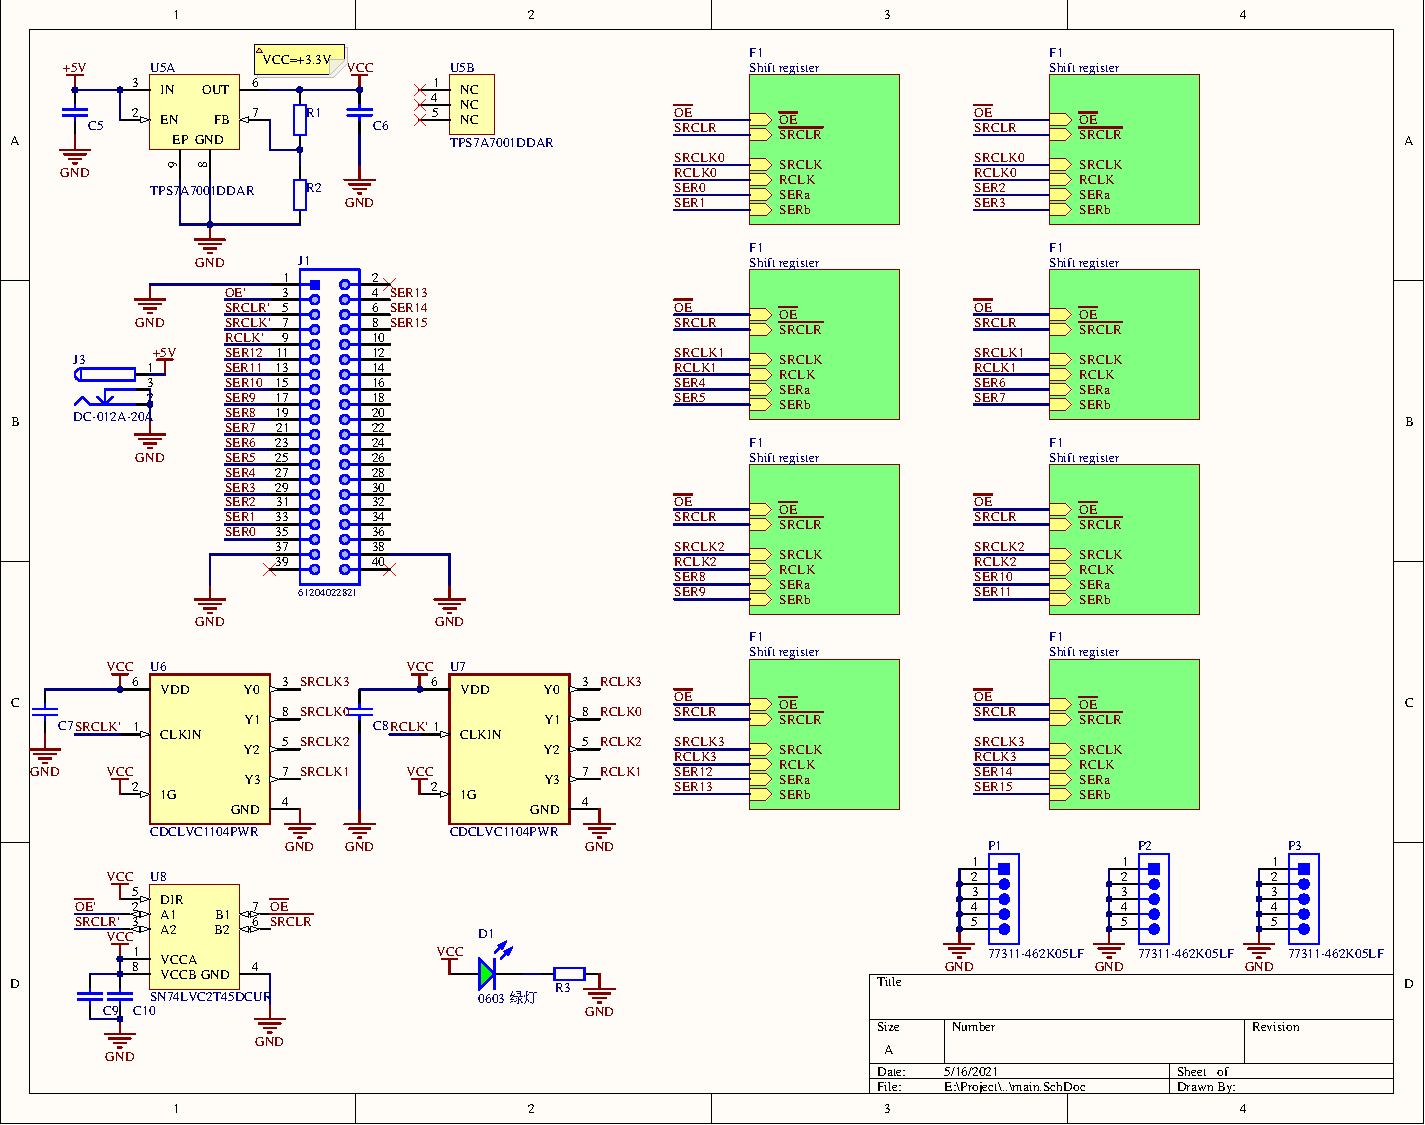
\includegraphics[width=\linewidth]{Figures/schdoc_1.pdf}
	\end{generalfig}

	\begin{generalfig}[htb]{原理图2}{fig:schdoc_2}
		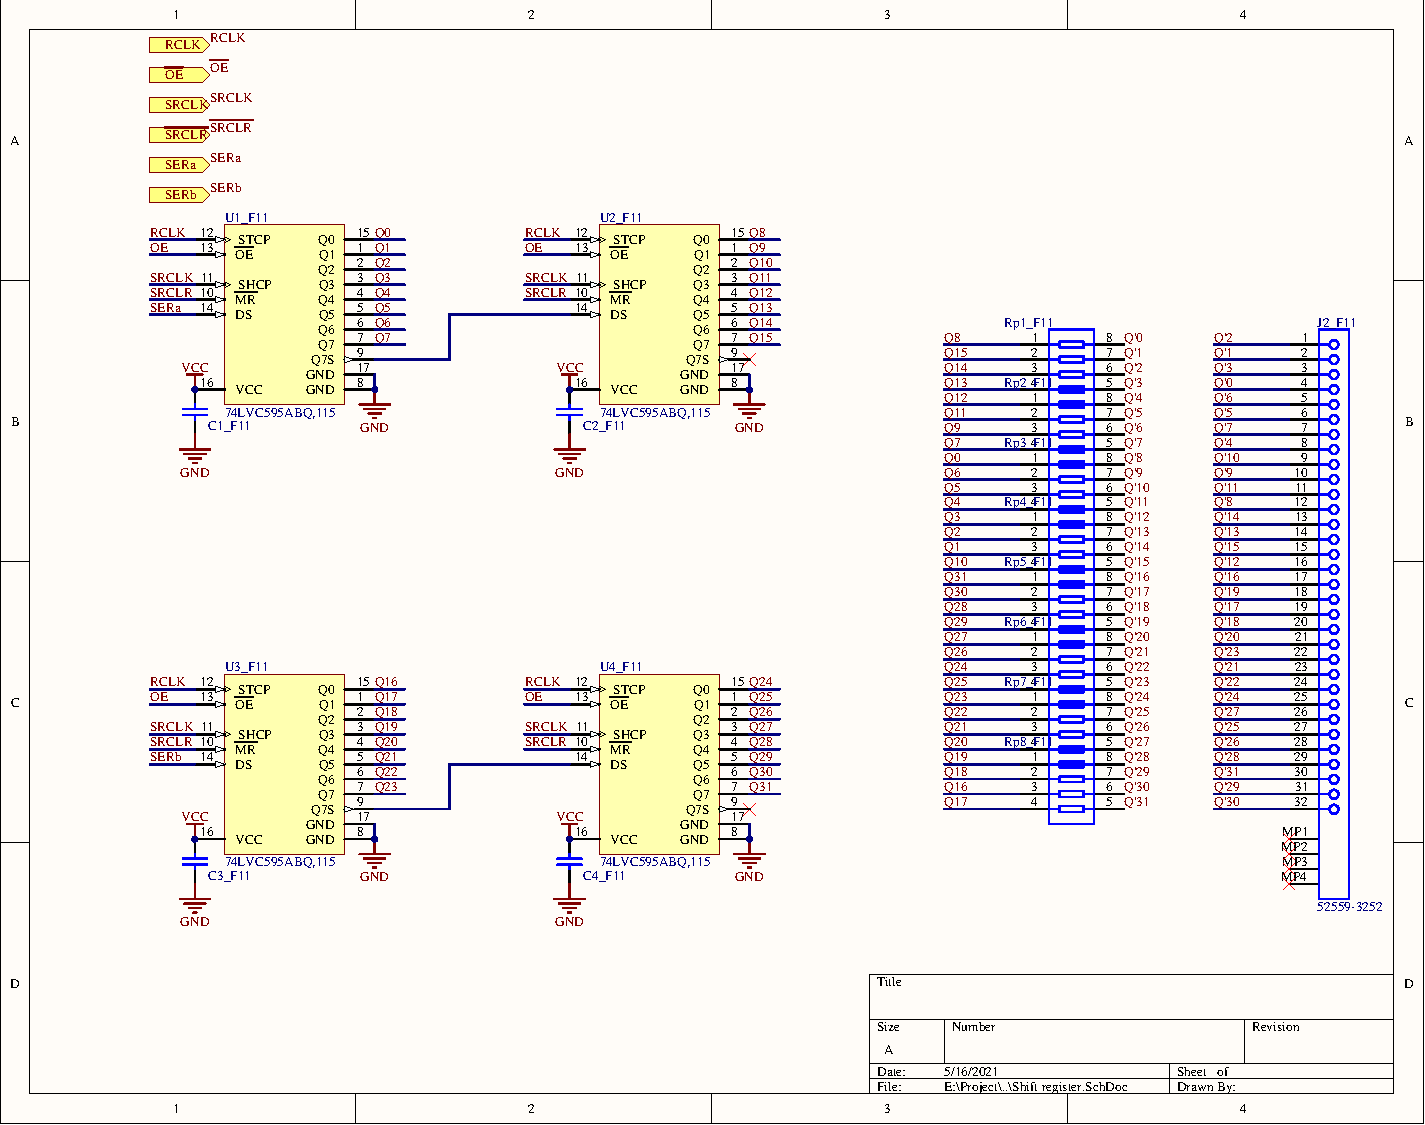
\includegraphics[width=\linewidth]{Figures/schdoc_2.pdf}
	\end{generalfig}

\end{appendices}

\end{document}




